%%
%% Jakub Žitný
%% Bachelor's thesis
%% Unix distribution portal
%%

% hidelinks remove colour boxes around hyperlinks
\documentclass[thesis=B,english]{FITthesis}[2013/04/26]

% packages
\usepackage[utf8]{inputenc} % LaTeX source encoded as UTF-8
\usepackage{graphicx} %graphics files inclusion
\usepackage{amsmath} %advanced maths
\usepackage{amssymb} %additional math symbols
\usepackage{dirtree} %directory tree visualisation
%\usepackage[export]{adjustbox}
%\usepackage[superscript,biblabel]{cite}
\usepackage[nonumberlist,numberedsection=autolabel]{glossaries}
%\usepackage{titlesec}

%%
%% GLOSSARIES
%%
\makeglossaries
\newglossaryentry{IaaS}
{
  name=IaaS,
  description={Infrastructure as a Service}
}
\newglossaryentry{SaaS}
{
  name=SaaS,
  description={Software as a Service}
}
\newglossaryentry{PaaS}
{
  name=PaaS,
  description={Platform as a Service}
}
\newglossaryentry{GUI}
{
  name=GUI,
  description={Graphical User Interface allows interaction with operating systems with clicking, icons and mouse without commands}
}
\newglossaryentry{PHP}
{
  name=PHP,
  description={programming language}
}
\newglossaryentry{ICT}
{
  name=ICT,
  description={Information and Communications technology}
}
\newglossaryentry{I/O devices}
{
  name=I/O devices,
  description={Input/Output devices such as printer or keyboard}
}
\newglossaryentry{API}
{
  name=API,
  description={Application Programming Interface}
}
\newglossaryentry{OS}
{
  name=OS,
  description={Operating System}
}
\newglossaryentry{REST}
{
  name=REST,
  description={Representational state transfer}
}

% other properties
\setcounter{secnumdepth}{5}
\setcounter{tocdepth}{2}
\newcommand{\myparagraph}[1]{\paragraph{#1}\mbox{}\\}

% header info
\department{Department of Computer Systems}
\title{Unix distribution portal}
\authorGN{Jakub} %(křestní) jméno (jména) autora
\authorFN{Žitný} %příjmení autora
\author{Jakub Žitný}
\authorWithDegrees{Jakub Žitný} %jméno autora včetně současných akademických titulů
\supervisor{Ing. Jan Trdlička Ph.D.}
\acknowledgements{I would like to take this opportunity to thank my supervisor Jan Trdlička who has been helping me with this project from the beginning.}

%% ABSTRACT 
\abstractEN{This project hopes to bring new way to distribute information about various operating systems -- especially multifarious Linux distributions but also other open-source systems. There are so many of them it is not easy to get to know or try out each one. The output of this work is design and implementation of web application which displays information about operating systems on well designed pages. These information come from automatic procedures scanning the inside of operating systems and the Internet. Besides displaying information, the website gives a chance for visitors to try out specific operating systems right in their browser. This project is inspired by ideas behind distrowatch.com -- a popular website providing updates and rankings of Linux distributions. }
\abstractCS{Tento projekt přináší nový způsob předávaní informací o různých operačních systémech. Především o různých Linuxových distribucích, ale i o jiných open-source systémech. Existuje jich nespočet a není snadné se o nich dozvědet více, případně si je vyzkoušet. Výstupem práce je návrh a implementace webové stránky, která zobrazuje informace o jednotlivých operačních systémech. Tyto informace získá automaticky prohledávaním nitra nainstalovaných systémů. Kromě toho mohou návštěvníci webu vyzkoušet vybrané distribuce přímo v prohlížeči. Tento projekt je inspirován populárním portálem distrowatch.com.}

\placeForDeclarationOfAuthenticity{Prague}
\declarationOfAuthenticityOption{1} %volba Prohlášení
\keywordsCS{distrowatch, cloud, infrastruktura jako služba, operační systémy, Linux, Unix, unix-like, distribuce, portál, vyzkoušení Linuxu, výběr Linuxové distribuce}
\keywordsEN{distrowatch, cloud, iaas, operating systems, Linux, Unix, unix-like, distributions, distros, website, try Linux distrobutions, software packages, screenshots \newpage}



\begin{document}

%% FIGURES
%%\newacronym{CTU}{Czech Technical University in Prague}
%%\newacronym{FIT}{Faculty of Information Technology}

%%
%% INTRODUCTION
%%
\begin{introduction}
\label{section:introduction}

Every once in a while people are born and people die. We do that for thousands of years and we are evolving. We make tools to help us live our lives easier and to dig deeper and deeper in the laws of nature. We seek the truth and the meaning of life. Sometimes we slow down or disobey our natural order. We fall, we blaspheme, we supress other people’s rights. But then again, we come together stronger and more connected. We resist and we earn the freedom and justice. Whereupon we make tools to work with the other tools easier and we find ourselves dedicated to religion, art, charity, humanities, science or technology. Some people do not, but others do dedicate their lives to improve the knowledge of mankind and to revamp new age with connected computers to the massive infrastructure called the Internet. \\

The 21st century’s powerful cloud applications provide great way of making our lives easier. Not just for ``IT people'', but for everybody. Even for monks or artists. However, people generally need to use computers just to do their work. They do not care about how these things work, they just need the stuff to be done. \\

Every computer, from little ereaders or smartphones in our pockets through the personal computers in our homes or workplaces to big datacenters managing stock markets, physics laboratories or space missions, needs to be driven by an operating system. The operating system is there to manage all the pieces of a complex system. Modern computers consist of processors, memories, timers, disks, mice, network interfaces, printers, and a wide variety of other devices. In the alternative view, the job of the operating system is to provide for an orderly and controlled allocation of these resources among the various programs competing for them \cite{tannenbaum}.\\

There seems to be common knowledge in all of the situations, when searching for the right operating system for the needed purpose. However, what if there was better choice for less experienced users or administrators? Not just in server datacenters, but even in ordinary life. In parents’ living rooms, in few-year-old students’ laptops or in girlfriends’ tablets. A lot of people are happy to choose their first Ubuntu as their new OS on low-end laptop. They browse the web, watch movies, write documents and emails and their computer is faster and more open than Windows. But hey, there is no intention to prefer one or another. The exact opposite. \\

People sometimes like to choose tools (their predecessors made up) to do their jobs. In this case, it would be great to create a tool to measure, test and observe various options of different operating systems for many purposes. Wouldn’t it be great, someday maybe, to be able in no time to compare hudreds of unix-like distributions or even try them in the browser without downloading and installing it? Wouldn’t it be even more perfect to be able to compare every aspect of newly shipped proprietary OS such as Windows or OS X? \\

Basics of these thoughts are going to be the essential part of the following work. The idea was initiated when comparing several Linux distributions at distrowatch.com -- the current number one ``comparator'' of operating systems. Read along to unveil the challenges this idea had met and defeated.
\end{introduction}

%%
%% Setting the scene
%%
\chapter{Setting the scene}
\label{chapter:setting_the_scene}

The bottom line of the previous thoughts is to create a website which will present complex information about operating systems, information coming from automated procedures. This creation will be the subject of this work, strutured as follows.

\section{Structure of the following chapters}

In the \hyperref[section:introduction]{Intruduction}, there were mentioned all motives regarding purpose and outcome of this work. They will be specified precisely in \hyperref[chapter:setting_the_scene]{this chapter}. \\

The \hyperref[chapter:analysis_and_design]{next chapter} deals with designed system from the grounds up. It focuses on all software features needed for the system to run. There is discussion about programming languages, frameworks and libraries that will be used and how will they communicate. \hyperref[chapter:implementation]{The chapter after that} covers the implementation. There are diagrams explaining the software architecture and examples of used components, \hyperref[section:testing]{testing} and \hyperref[chapter:production]{production} environment. \\

There are also few appendicies, to extend the information in this work, containing screenshots of created website and domain models.

\section{Functionality}

Let us call the would-be website ``The New Distrowatch'' (TND) and start with specific functions it should provide.

\subsection{Information about operating systems}

TND will present various information about unix-like systems similar to those available at distrowatch.com. These information will be produced automatically and this will be its main asset. Users will be able to search for desired distribution and TND will show them detailed information about it. For example screenshots of GUI, links to the origin and website, mirror sites with downloadable installation media, kernel type and version or installed software. On the other hand, administrator, from his point of view, will be able to add new distribution just by uploading installation media. The backend system will install it, automatically process the installed system and found information will be added to the database.

After administrator's submission the backend side will install the operating system from submitted installation media. Installed system will be stored as virtual disk image and scanned by automated procedures for all the information later presented to users. These procedures will be modular parts of the backend system.

Since the automated installation process is not possible to implement across all the present and future operating systems, the backend system should be able to guide administrator through manual installation step by step or to accept pre-installed images of operating systems that some OS-makers provide.

Backend system will be also able to browse reliable sources on the Internet for aditional information. For example, if it fails to retrieve the screenshot of specific distribution, one of the sources could be scanned for presence of desired screenshot.

\subsection{Operating system in the cloud}

Website visitors will be able to launch specific distributions and try out features of each system and platform. Backend will start a distribution in virtual environment on user's request. After the system is successfully launched, the website will display a remote desktop console attached to the launched system. In addition to that, users will also be able to connect to the system through SSH from command line or through VNC remote desktop client.

Distributions, launchable from the website, will be created as instance of virtual disk image, previously installed after administrator's submission, in the cloud. Before launching, images have to be modified for presence in the cloud.

\subsection{Other functionality}
\label{section:other_functionality}
In order to deliver more complex browsing experience to the user, TND website should be displaying additional content besides the specific operating system information. These information will be mainly updates similar to those at distrowatch.com and published news from ICT industry in general.

Whole system will be designed in a way that will enable future modifications and addidtions. Some of them will also be outlined in following chapters. TND could be unique web portal with concentrated information about operating systems and the right place to consider a unified way of offering installation media in different formats (the os-centric instance of sourceforge). TND could also use the pre-installed images for deployment in business IaaS cloud environments.

The system will be implemented in a way that will easily enable future improvements, mainly in the backend side. For example, users could be interested in details about different versions of Microsoft Windows. However, these are not that easy to automate. Thus, they will not be part of this work. On the other hand, thanks to desired modularity of backend, they could be easily implemented in the future and revamp the TND offerings for users.

\section{Principles}
\label{section:principles}
The purpose of this work is design and implementation of system with previously mentioned capabilities. It is going to do analysis in almost all of the IT-related fields which are relevant in building the system from the grounds up and bringing it to the public. This work tries to be clear, open and precise as it is possible.

The result of this project -- the TND website -- could be real benefit for the Linux communities, for beginners and also for advanced users looking for detailed differencies between specific operating systems. Mere mortals outside the IT industry could also find there lot of information about popular Linux distributions, such as Ubuntu, Fedora or Mint. Why their friends recommended this distro rather than the other one. Later, maybe, they could also find there differences between Windows versions and editions. That could easily satisfy even more curious enthusiast.

\section{Comparsion to distrowatch.com}

Many ideas behind this work are inspired by popular, almost 12-year-old website called Distrowatch. It was one of the first projects providing detailed information about various Linux distributions and other operating systems. Visitors can find there screenshots, links to websites, software, software versions and stuff like that. There are almost one hundred contributors today who help with data about various systems \cite{dw_about}.

Now, there is no official record of how information at distrowatch.com are produced. However, given the ratio of static to dynamic information, automated retirieval of information could be higher. The other disadvantage of this website is its look and graphical design. Subjectively.

Since this work will have similar mission as Distrowatch, it is going to offer refined way of collecting and displaying the content. It is also going to add new funcionality for potential visitors. Otherwise, it will not make any sense. If this project will work itself up, it could also provide platform for other ideas easing the people's work.


%%
%% ANAL AND DESIGN
%%
\chapter{Analysis and design}
\label{chapter:analysis_and_design}

To provide a clear picture of designing each part of TND, the system will be split into frontend and backend, frontend being the client website which will interact with users and backend being server-side application, automatically processing requests, mining data and executing tasks. They will communicate with each other.

First, the basic tools for implementation will have to be determined and one of them is programming language.

\section{The preferred programming language}

TIOBE Programming Community Index measures the popularity of programming languages monthly, based on the number of search engine results for queries containing the name of the language \cite{tiobe_def}. Top ten results for April 2013 in ascending order are following: C, Java, C++, Objective-C, C\#, PHP, (Visual) Basic, Python, Perl and Ruby \cite{tiobe_res}.

Programming language that is going to be chosen for this work should be able to acomplish its core goals. It should also provide some higher level frameworks built on top, to simplify the web development process. It should also be~well-documented. All mentioned languages satisfy the first ability, however, not all of them suffice the latter, namely C, C++, Objective-C, (Visual) Basic and Perl.

Since this work will not be dependent only on the web layer, the preferred language should be capable of doing ``the backend work''. It could be a scripting language, however, it should provide great number of libraries built on top. Since ``the backend work'' would sometimes need to be done quickly by tiny executables, the list will have to be reduced by Java and C\#.

Ruby has the benefit of not lagging by new releases. Unlike Python, which came transformed to version 3 in 2008 and still have less users and contributors using it. On the other hand, in favor of Python becoming the preferred choice are the bigger number of frameworks and libraries easying the work and the author's experience with it. \\

So ``the chosen one'' is Python in the newest stable release -- 3.3, however, the frontend will be implemented in PHP due to security and easiness issues that are detailed in the following chapter.

\section{Components}

This projet divides into frontend (client) and backend (server) side. However, additional fractions for this chapter are needed in order to be as clear as possible. The backend part will be splitted into three components.

\begin{enumerate}
	\item \emph{Automated procedures} will be the common name for the backend modules fulfilling the automated work.
	\item To the furthest part of backend where instances of operating systems will be launched, this chapter will be referring as \emph{Cloud gate}.
	\item The last one, confusingly being in the exact middle of all components, will be called \emph{Controller} and it will link the frontend and backend.
\end{enumerate}

\subsection{Frontend}

Frontend website is where all the produced information will be presented to visitors. In order to show so many data and still be clear and cool and also to offer difference to distrowatch.com a toughtful graphical design have been proposed.

\subsubsection{Graphical interface}

Since the graphical design is to be done by skilled designer, two students from CTU's Faculty of Architecture were requested to sketch their views of how TND should look like. The final look of the website is shown in the \hyperref[TODO]{Appendix B}.

\myparagraph{Menu}

This work is not just about the website, so there will not be a discussion about web-designing techniques nor about JavaScript libraries. Let's just consider the web done and describe the looks of TND in short.

Menu of TND webside consists of following pages.

\begin{itemize}
	\item \textbf{Home} displays current top rating distributions and last few news and updates. 
	\item \textbf{Distros} list all operating systems that are stored in database. After clicking on one of them, the ``profile page'' of that system is shown.
	\item \textbf{News} list all news sorted by date.
	\item \textbf{Updates} list all updates sorted by date. 
	\item \textbf{About} tells about this project and shows contact information and e-mail form.
\end{itemize}

\subsubsection{Languages and frameworks at frontend}

In the \hyperref[TODO]{second chapter}, Python was chosen as the preferred programming language. However, PHP and frameworks bulit on top of it seem to be the most used tools to create reliable websites.

BuiltWith Trends, web technology statistics website which provides free information about the most popular technology used on the web \cite{builtwithfaq}, calculated on April 5th 2013 frameworks distribution from the top million websites on the Internet. PHP is the most popular framework in the BuiltWith list, although many sites report PHP usage even if it is not being used \cite{builtwithfaq}. Popular portal phpzag.com \cite{mysitecostphpzag} lists the top 5 frameworks of the year 2012 built on top of PHP -- Yii, CodeIgniter, Zend, CakePHP and Symfony \cite{phpzag}.

Let us look at the competing platforms for frontend one by one. The first choice would be certainly Python and the most widely used Python web framework -- Django. The other ones supports the idea of implementing the frontend in a classic way -- in PHP. 

\myparagraph{Django (Python)}

Django is a high-level Python Web framework that encourages rapid development and clean, pragmatic design. Developed by a fast-moving online-news operation, Django was designed to handle two challenges: the intensive deadlines of a newsroom and the stringent requirements of the experienced Web developers who wrote it. It lets you build high-performing, elegant Web applications quickly. Django focuses on automating as much as possible and adhering to the DRY principle \cite{django}.

\myparagraph{Symfony (PHP)}

Symfony is a PHP Web Development Framework that focuses on security and the ease in building robust applications. It follows the MVC pattern and implements the object-relational mapping with Doctrine2 to reduce programmers need to access to database directly. 

\myparagraph{Zend (PHP)}

Zend Framework 2 is an open source framework for developing web applications and services using PHP 5.3+. It is one of the oldest and biggest among competitors. Zend Framework 2 uses 100\% object-oriented code and utilises most of the new features of PHP 5.3, namely namespaces, late static binding, lambda functions and closures. Zend Framework 2 evolved from Zend Framework 1, a successful PHP framework with over 15 million downloads. \cite{zend} Zend is often used on smaller project that are not worth the trouble of having such a big framework. \\

Well, this part is not that important, so popularity, documentation, security and author's experience with it are going to ``vote'' for using Symfony2 framework. However, the chosen ones could be also many others, such as Nette or even Java EE.

\subsubsection{Designing the web in Symfony2}

Symfony2 also offers a number of libraries that could ease one's implementation. Libraries for the Symfony2 framework are called bundles and few of them was considered to come handy and they were tested.

\begin{itemize}
	\item \emph{FOSUserBundle} adds support for a database-backed user system in Symfony2. It provides a flexible framework for user management that aims to handle common tasks such as user registration and password retrieval \cite{fosuserbundle}.
	\item \emph{FOSFacebookBundle} provides a Symfony2 authentication provider so that users can login to a Symfony2 application via Facebook. Furthermore via custom user provider support the Facebook login can also be integrated with other data sources like the database based solution provided by FOSUserBundle \cite{fosfacebookbundle}.
	\item \emph{RedisBundle} integrates Predis and phpredis libraries communicating with Redis message queue into Symfony2 applications \cite{redisbundle}.
\end{itemize}


\subsubsection{Running the website}

Let us consider the frontend implemented again. In order to run it and do the work on backend, there need to be chosen webserver and database for it.

This year's active webservers are popular in following order \cite{webserver_usage}:
\begin{enumerate}
	\item Apache 55,50\%
	\item nginx 11,90\%
	\item Microsoft 11,35\%
	\item Google (GWS) 8,04\%
\end{enumerate}

TND will use the most popular webserver without any doubts. Database design is covered in the next chapter, the chosen engine is PostgreSQL.

\subsection{Automated procedures}

Several procedures that will bring automated approach to the process of manipulating and scanning operating systems are the core of this work. They are one of the reasons this work is relevant and not just the old distrowatch.com with new graphic design.

Having chosen Python as the preferred language, these procedures will be written in popular framework built on the top of Python -- Django. Thanks to Django, these procedures could be easily implemented as modules. Modules in Django are called apps. They will be launchable from the admin interface, called Admin Console, implemented as a Django app, too.

To sum backend's automated work up, let's look at how system would be filled with operating systems. There should be as little human interaction as possible. 

\begin{enumerate}
	\item At first, administrator will manually add the installation media of desired operating system.
	\item Then the installation app will attempt to install it in virtualization environment and save it as virtual disk image.
	\item Another app -- the scanner -- will then scan the image for information and collect them in database.
	\item The image will also be modified for use in IaaS cloud environment. This would be done by script called vdpatch.
\end{enumerate}

If the automatic installer fails to install the system, backend will start the guided administrator's manual installation process. This is very important because of many systems' installation process uniqueness. One of the ways to simplify the installation process handling is to use pre-installed virtual image that some maintainters provide.

Following sections discuss each of the automated procedures in more detail.

\subsubsection{Operating systems installation}

Automated installation of specific operating system is very difficult task. There are few projects trying to offer a general approach for wide range of distributions. There are also few tools that solved it for a specific distribution and its derivatives. Let's look at them.

\myparagraph{FAI-project}

FAI is a non-interactive system to install, customize and manage Linux
systems and software configurations on computers as well as virtual
machines and chroot environments, from small networks to large
infrastructures and clusters. It's a tool for mass unattended Linux
installation. You can take one or more virgin systems, turn on the
power, and after a few minutes, the systems are installed, and
completely configured to your exact needs, without any interaction
necessary. Thus, it's a scalable method for deploying and updating a
Beowulf cluster or a network of workstations unattended with little
effort involved. FAI uses the Debian distribution and a collection of
shell and Perl scripts for the installation process. Changes to the
configuration files of the operating system are made by cfengine,
shell and Perl scripts \cite{fai_about}.

FAI supports Red-Hat, some of its derivatives, such as Fedora, Oracle, CentOS or Scientific Linux, Debian and its derviatives, such as Ubuntu and SUSE. The official project website list the main features \cite{fai_home}:

\begin{itemize}
	\item centralized deployment and configuration management,
	\item installs XEN domains, VirtualBox and Vserver,
	\item easy set up of software RAID and LVM,
	\item full remote control via ssh during installation,
	\item integrated disaster recovery system,
	\item every stage can be customized via hooks.
\end{itemize}

\myparagraph{M23}

M23 is distribution system that claims to be able to install and administer Debian, Mint, Ubuntu, openSUSE, Fedora and CentOS distrubutions of Linux from web browser. \cite{m23}

\myparagraph{Anaconda, Kickstart and Cobbler}

Anaconda is the installation program used by Fedora, Red Hat Enterprise Linux and some other distributions \cite{anaconda}.

Kickstart provides a way for users to automate a Fedora installation. Kickstart files can be kept on a single server system and read by individual computers during the installation. This installation method can support the use of a single kickstart file to install Fedora on multiple machines, making it ideal for network and system administrators \cite{kickstart}.

Cobbler is a Linux installation server that allows for rapid setup of network installation environments. It glues together and automates many associated Linux tasks so you do not have to hop between many various commands and applications when deploying new systems, and, in some cases, changing existing ones. Cobbler can help with provisioning, managing DNS and DHCP, package updates, power management, configuration management orchestration, and much more \cite{cobbler}.

\myparagraph{YaST, AutoYaST}

YaST is the installation and configuration tool for openSUSE and the SUSE Linux Enterprise distributions. It is popular for its easy use, attractive graphical interface and the capability to customize your system quickly during and after the installation. YaST actually stands for Yet another Setup Tool. YaST can be used to configure your entire system. Setup hardware, configure the network, system services and tune your security settings. All these tasks can be reached from the YaST Control Center \cite{yast}.

AutoYaST2 is a system for installing one or more SUSE Linux systems automatically without user intervention. AutoYaST2 installations are performed using an AutoYaST profile with installation and configuration data. That profile can be created using the configuration interface of AutoYaST2 and can be provided to YaST2 during installation in different ways \cite{autoyast}. \\

To sum things up, most of these projects started up because people demanded tools for mass deplyment of specific system. For example a administrator of school classrooms with computers needed to install the same for all computers and he wanted to make it as quickly as possible. Now, this is not exactly the thing this project needs because it will install every system just once and the initial configuration these tools require is the thing we are trying to solve. However, specific systems have specific patterns in terms of setting them up and these tools, especially the official ones such as YaST or Kickstart, offer great way to be aware of them.

After reviewing available tools that already tried to solve automating the installation, the case of designing the \emph{installer} should be more clear. It will be taught to install currently widely used open-source systems by series of scripts. So after new system or distribution is submitted, the script should try to guess its nature or predecessors and if it matches, the app will apply it's taught mechanism.

\subsubsection{Virtual disk image modification}

The \emph{vdpatch} tool will be scripted solution for decompressing virtual disk image, chrooting into it and executing specific modifications. Among these modifications is assigning public IP address, enabling SSH connections, installing tools for virtual environments, etc. When finished, modified image will be saved as ready to be deployed for user.

\subsubsection{Quest for information}

Automated scanning of the internals of the image will be done using chroot utility, too. When chrooted, it will collect information about the system and save it to database. The collection of data will consist of kernel type and version, bootloader, package management system, installed software and things like that.

\subsubsection{Quest for screenshots}

Screenshots of GUI are one of the most interesting details for beginners. Not all operating systems have GUI so the quest for screenshots will be optional. Administrator will have to trigger this procedure. The easiest way to obtain a screenshot of system is to launch it with KVM and retrieve the screenshot at specific time from the virtualization environment. It is possible.

On the other hand, creating screenshots manually is really hard to reproduce using automated process. When reviewer is taking screenshots of launched applications and layout of various parts, the automated procedure would have to be very smart to reproduce the ``clicks'' that creates the esthetic layouts of good screenshots.

\subsubsection{Backup information}

There will also be an app, which will browse the web for additional information about distributions. It will import data from a number of trusted sites with similar content, e.g. Wikipedia, Distrowatch or Screenshot Directory.

A lot of information will be retrieved from distrowatch.com, in order to make the TND web filled with information from the beginning. They have already great descriptions of operating systems and it should not be wasted. Of course, the reference to original text will be published. Another source -- the Screenshot Directory -- is a project by Chris Haney located at \url{http://www.chrishaney.com/?linux} that regularly publishes screenshots from new versions of Linux distributions.

\subsubsection{Admin Console}

All the automated procedures will be launched automatically by backend controller after administrator's submission of new operating system. The place where the administrator can do such thing (and many others) is called Admin Console -- Django app with web interface.

\subsection{OS in a browser}

We want to enable users to try out desired distributions directly in browser. That could be useful for beginners to try different GUIs they have heard about and for advanced users, too.

The ideal result would be to have special button in every operating system's or distribution's page for deployment, and after pressing it, new page with VNC web console will be opened and SSH credentials will be offered to user.

There are two ways to achieve this goal. The first is using KVM virtualization engine with libvirt interface and the other is using more complex but more powerful IaaS cloud platform. Both are described in the following sections.

\subsubsection{Virtualization environment}

The less complex solution to present launched operating systems to users is to use virtual environment. One of the most used ones and also open-source is KVM -- the Kernel-based Virtual Machine. It is available for Linux and FreeBSD. Together with virtualization library libvirt built on top of it, it is easy to create, launch and delete virtual machines. These machines would be launched with virtual disk of a specific distribution, created earlier.

Public IP adresses will be assigned to these virtual machines, VNC and SSH connection will be enabled on them and when user clicks the button for deployment on the web, this system will be launched and access to it will be sent to user.

\subsubsection{IaaS cloud}

The other way is to implement private infrastructure cloud that will easily communicate with backend system and after users' attempt to deploy specific distribution, it will be launched on predefined virtual hardware. But first, let's look at the cloud computing and explain what infrastructure cloud means.

There are essentially three ways in which a business may replace traditional in-house systems with cloud computing. Specifically, the available options are:
\begin{enumerate}
	\item Software as a Service,
	\item Platform as a Service,
	\item Infrastructure as a Service.
\end{enumerate}

All of the above involve a cloud vendor supplying servers on which their customers store data and run applications. However, the differences between SaaS, PaaS and IaaS concern the level of control that a business has over the applications they use, how these applications are created, and the type of hardware on which their applications are run.
When business opt for SaaS they can only run those applications that their cloud supplier has to offer. When they opt for PaaS they can create their own applications but only in a manner determined by their cloud supplier. And when they opt for IaaS they can run any applications they please on cloud hardware of their own choice \cite{cc_guide}.

To use the IaaS cloud privately would in this case mean that we will have the system behind our system and we will provide users with access to it, but without the option to manipulate with it. It will be IaaS for this project, but for users it will be on the edge between the platform and sofware as a service cloud. Let us list some of the most popular IaaS cloud providers.

\myparagraph{Amazon Web Services}

Amazon Elastic Compute Cloud (Amazon EC2) is a web service that provides resizable compute capacity in the cloud. It is designed to make web-scale computing easier for developers. Amazon EC2’s simple web service interface allows you to obtain and configure capacity with minimal friction. It provides you with complete control of your computing resources and lets you run on Amazon’s proven computing environment. Amazon EC2 reduces the time required to obtain and boot new server instances to minutes, allowing you to quickly scale capacity, both up and down, as your computing requirements change. Amazon EC2 changes the economics of computing by allowing you to pay only for capacity that you actually use. Amazon EC2 provides developers the tools to build failure resilient applications and isolate themselves from common failure scenarios \cite{aws}.

\myparagraph{OpenStack}

OpenStack is a cloud operating system that controls large pools of compute, storage, and networking resources throughout a datacenter, all managed through a dashboard that gives administrators control while empowering their users to provision resources through a web interface \cite{openstack}.

\myparagraph{Eucalyptus}

The Eucalyptus Cloud platform is open source software for building AWS-compatible private and hybrid clouds. It pools together existing virtualized infrastructure to create cloud resources for compute, network and storage. The Eucalyptus Cloud can dynamically scale up or down depending on application workloads and is uniquely suited for enterprise clouds, delivering production-ready software that supports the industry-standard AWS APIs, including EC2, S3, EBS, and IAM. The benefits are highly efficient scalability, organization agility, and increased trust and control for IT \cite{eucalyptus}.

\myparagraph{OpenNebula}

OpenNebula.org is an open-source project developing the industry standard solution for building and managing virtualized enterprise data centers and enterprise private clouds \cite{opennebula}. \\

We could set up one of these systems to launch desired operating systems for us without the need to implement virtualization and resources distributing. The backend system would only send commands to the private cloud via ``cloud gate'' and everything will be taken care of. \\

The decision to select a ``winner'' or the most dominant private IaaS system is not a simple one. Although most of the systems share and meet a common objective (instantiation of virtual machines at large scale), they vary significantly when it comes to performance in the various criteria. Generally, OpenNebula targets science communities thanks to features such as contextualisation and support of distributed file systems. Enterprises tend to opt for more robust and stable solutions and hence may be attracted to Eucalyptus. Cloud enthusiasts and adventurers may be tempted into OpenStack due to its promising future and largest background \cite{klepac}.

OpenStack and Eucalyptus can be controlled by similar command line tools and also via REST API. The final decision would still be dependent on the resources we would have and on the level of integration to this project. However, let us make the choice and say we would be happy to use OpenStack.

\subsection{Controller}

Backend system should have the central processing unit, right? It has to listen somewhere for interaction with frontend and it must have the access to the web database so the scanned information could be saved there. This part of backend will be called Controller and as we have decided earlier, it will be implemented in Django, built on top of Python.

All of the automated procedures from previous chapter will be implemented inside this. Of course, there will be a way to launch all the procedures from command line, as mentioned \hyperref[TODO]{earlier}.

Backend system and frontend website will both be launched on separated machines. Backend will be run via Django built-in webserver.

\section{Communication between frontend and backend}

When user toggles the operating system deployment, frontend should pass the information to the backend who would execute the task asynchronously. Passing these and other information -- communicating -- between frontend and backend have to be secure, fast and precise. In order to choose the right communication method, some of them were tested and compared. \\

Let's look at possible data that will be sent through this communication canal.

\begin{itemize}
	\item When user is browsing the TND website and wants to deploy specific operating system, frontend enables him to send a request to the backend where the system would be launched and the information about how to connect to launched instance would be returned to user. This should be done without user's waiting for page refresh.
	\item When administrator submits new installation media or image via Admin Console, backend is supposed to execute active apps to process it (e.g. scan for information or screenshots) and Admin Console would show the output of processing executing tasks.
\end{itemize}

Popular communication methods related to web and Python are following.

\subsection{Via HTTP}

The easiest way to send a task from the web interface (client) to backend is to send data directly via HTTP protocol. To send it without refreshing a page it should be done asynchronously and result should be polled or pushed when execution finishes. This could be done via Ajax calls from client-side JavaScript.

\myparagraph{XML-RPC}

XML-RPC is a Remote Procedure Calling protocol that works over the HTTP. An XML-RPC message is an HTTP-POST request. The body of the request is in XML. A procedure executes on the server and the value it returns is also formatted in XML. Procedure parameters can be scalars, numbers, strings, dates, etc.; and can also be complex record and list structures \cite{xmlrpc}.

\myparagraph{RPyC}

RPyC is a transparent python library for symmetrical remote procedure calls, clustering and distributed-computing. RPyC makes use of object-proxying, a technique that employs python’s dynamic nature, to overcome the physical boundaries between processes and computers, so that remote objects can be manipulated as if they were local \cite{rpyc}.

\myparagraph{SOAP}

SOAP is a lightweight protocol for exchange of information in a decentralized, distributed environment. It is an XML based protocol that consists of three parts: an envelope that defines a framework for describing what is in a message and how to process it, a set of encoding rules for expressing instances of application-defined datatypes, and a convention for representing remote procedure calls and responses. SOAP can potentially be used in combination with a variety of other protocols; however, the only bindings defined in this document describe how to use SOAP in combination with HTTP and HTTP Extension Framework \cite{soap}.

\subsection{Via message queue}

Messaging enables software applications to connect and scale. Applications can connect to each other, as components of a larger application, or to user devices and data. Messaging is asynchronous, decoupling applications by separating sending and receiving data \cite{rabbitmq_official}.

\myparagraph{Redis}

Redis is an open source, BSD licensed, advanced key-value store. It is often referred to as a data structure server since keys can contain strings, hashes, lists, sets and sorted sets.

You can run atomic operations on these types, like appending to a string; incrementing the value in a hash; pushing to a list; computing set intersection, union and difference; or getting the member with highest ranking in a sorted set.

In order to achieve its outstanding performance, Redis works with an in-memory dataset. Depending on your use case, you can persist it either by dumping the dataset to disk every once in a while, or by appending each command to a log.

Redis also supports trivial-to-setup master-slave replication, with very fast non-blocking first synchronization, auto-reconnection on net split and so forth.

Other features include Transactions, Pub/Sub, Lua scripting, Keys with a limited time-to-live, and configuration settings to make Redis behave like a cache.

You can use Redis from most programming languages out there \cite{redis}.

\myparagraph{Rabbit MQ}

RabbitMQ is a messaging broker -- an intermediary for messaging. It gives  applications a common platform to send and receive messages. It offers a variety of features to trade off performance with reliability, including persistence, delivery acknowledgements, publisher confirms, and high availability. \cite{rabbitmq_official}.

RabbitMQ is a fast, reliable, open source queueing option. It's developed in Erlang, a functional language with a reputation for distributed, high availability, fault tolerant apps. It presents itself as a separate daemon -- much as Apache, Passenger, memcached, or MySQL. Using it isn’t difficult, and, of course, programmers can use it from a multitude of languages so if they want to push in items from PHP and pull them out to be processed with something else (or vice versa) it's ideal. RabbitMQ can be used as a hub for communication between all of your processes \cite{rabbitmq}.

\myparagraph{Celery}

Celery is an asynchronous task queue based on distributed message passing. It is focused on real-time operation, but supports scheduling as well. The execution units, called tasks, are executed concurrently on a single or more worker servers using multiprocessing, eventlet, or gevent. Tasks can execute asynchronously (in the background) or synchronously (wait until ready) \cite{celery}.

\myparagraph{Huey}

Huey is a task queue for Python and Django that supports multi-threaded task execution scheduled periodically or at specific time. It is lightweight library with similar use as Celery. It has better support for Python 3, easier setting up but less possibilities \cite{huey}. \\

Since the Redis project is the best maintained solution for cross language asynchronous communication and also has great foundations behind, it has been chosen. The Redis message queue will be placed between frontend and backend.

%%
%% IMPLEMENTATION AND TESTING
%%
\chapter{Implementation}
\label{chapter:implementation}

Having discussed all the possible scenarios and implementation features, it is much more easier to create desired application.

To sum things up again, there will be two separated parts: frontend and backend. Frontend is built on top of Symfony2 PHP framework. Backend is Python 3 and Django project, it has administration interface called Admin Console and modules that carry business logic tasks, called apps. They implement automated procedures and communication with private IaaS cloud. Frontend and backend communicate through Redis message queue with messages having specific format, detailed in section \hyperref[section:communication]{Communication}. This is the architecture design shown in \hyperref[TODO]{figure 3.1}.

Domain models that explain how important parts of the implementation work are placed in Appendix C.

\begin{figure}[h!]
	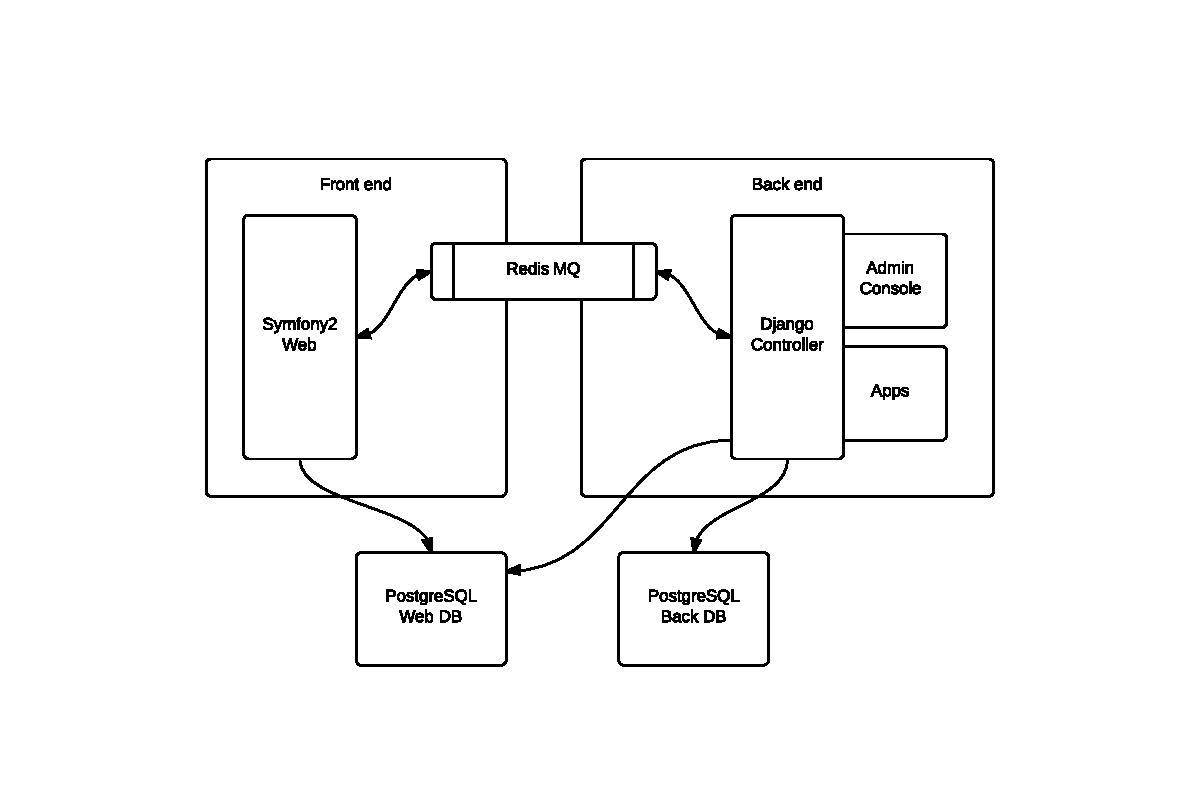
\includegraphics[trim=3.2cm 2cm 3cm 2.5cm, clip=true, totalheight=260pt]{images/tndw-arch.pdf}
	\caption{Architecture diagram}
	\label{fig: tndw-arch}
\end{figure}

%TODO \section{Use cases}

\section{Frontend}

Frontend is implemented in one bundle, which is the Symfony title for module. Frontend follows the Coding Standards of Symfony2 framework \cite{symfony_conventions}, Model-view-controller pattern and Three-tier architecture. MVC is realized easily thanks to Symfony structuring of the bundle. It divides the presentation layer consisted ot HTML templates an JavaScript code, router for dispatching requestes and object-relational mapping of Entities to the database into separate places.

Templating system in Symfony allowed us to create well-designed and organised graphic layout. Better viewing experience and responsive design approach is done by CSS3 style sheeting and jQuery JavaScript libraries.

Connection to the database is implemented via Object-relational mapping engine called Doctrine.

Registered users can deploy specific operating systems in the cloud and the acces to the launched systems in the browser is done using the Flash VNC console FlashLight VNC.

Most of the programming in the frontend have been focused on displaying data from database. Class layout is described in Appendix C.

\section{Backend}

Backend of the project consist of mentioned components displayed in diagram 3.1 -- Django controller, Admin Console and apps.

Backend is designed to be accessed via Admin Console. Every app though, could be also run from the command line. Scheme of the internals is shown on domain diagrams in Appendix C.

\subsection{Connection to the cloud}

Django controller is a multiprocess deamon module that communicates with frontend. It captures messages about users' requests to deploy operating systems and takes actions. If everything is all right, it deploys specific operating system in the cloud and returns necessary information to frontend. It would be best to implement this feature with OpenStack IaaS cloud service, however, the lack of computing and storage resources forced us to use different solution. Details about OpenStack and reasons why it is the best solution for this case are described in Chapter 2. The backup plan is to use a ``gate'' with access to Deltacloud REST API of T-Mobile CZ IaaS cloud project called T-Mobile Cloud. It is available at \url{cloud.t-mobile.cz} and it offers creation and management of virtual servers. Through this API, applications can manage servers in IaaS cloud. We use Deltacloud API in this project's backend, so it will be easy to change T-Mobile Cloud for other IaaS public or private provider (such as OpenStack).

To summarize, after user's request for deplyment of specific operating system on TND website, backend controller will deploy the system in the T-Mobile Cloud through Deltacloud REST API, for the time being. However, backend is prepared for this to be easily changed. T-Mobile cloud is a paid service.

\subsection{Automated procedures}

Automated procedures are implemented thanks to several classic Unix command line tools, Qemu command line tools and Python libraries. Among them are chroot, kpartx, losetup, parted, dmsetup, vgscan, vgchange, qemu-img and qemu-nbd.

The prototype application is called vdpatch and it is a BASH script. It's few hundred lines of code long and it can be viewed at \url{https://github.com/jakubzitny/tndw-controller/blob/master/vdpatch.sh}. It converts virtual disk images from and to different formats. Besides that, it can modificate the internals of images and scan for various information inside the image. It works like this: First, the script recognizes the format of the input virtual disk image and it converts it to raw format so it can be mapped and mounted as a block device. The recognition and conversion is done using qemu-img and qemu-nbd tools. After that, the image is mapped and mounted as a block device using kpartx, vgscan, vgchange and losetup utilities. When the image is mounted, the script sets up the chroot environment on top of the operating system installed on the input image. Most of the components and internals of the operating system can be scanned or changed in this environment. After desired work there is done, vdpatch script ensures proper disconnection and cleans up the environment. \\

Obtaining ``backup'' information from trusted sources on the Internet is done thanks to Python libraries lxml and requests. Scanning the sources and parsing data is done by multiprocessing units and saved into database via Django ORM Models interface.

\section{Communication}

Redis have been selected for this project as the best message broker available for this kind of work. It has well defined format of communication, which consists of correlation id (CID), exit code (EXT) and either command string (COM) or the result of command (ANS). The format is following.

\begin{center}
	\begin{verbatim}
	CID:EXT:COM/ANS
	\end{verbatim}
\end{center}

Simplified version of communication from frontend's deployment request to deployment itself is displayed on sequence diagram 3.2.

\begin{center}
\begin{figure}[h!]
	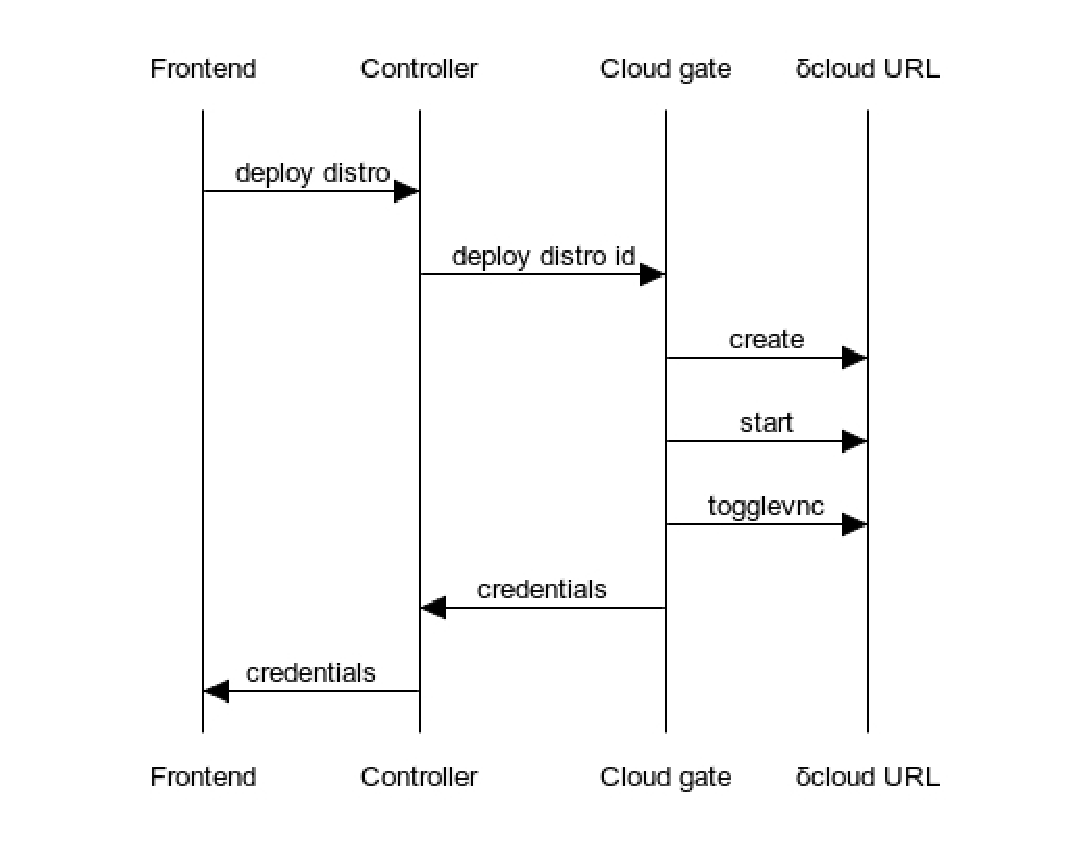
\includegraphics[totalheight=295pt]{images/sequence.pdf}
	\caption{Communication between frontend and backend}
	\label{fig: sequence}
\end{figure}
\end{center}

Messages to Redis are sent when:

\begin{itemize}
	\item user asks to deploy specific distribution in the cloud,
	\item Ajax is asking whether selected distribution has been deployed,
	\item admin submits tasks to be performed in backend.
\end{itemize}

\section{Testing environment}
\label{section:testing}
Testing environment is simulating the would-be production environment. It has two virtual servers. The first one runs Apache web server with frontend, PostgreSQL server with phpPgAdmin and Redis server with phpRedisAdmin. Second one runs Django webserver, controller and Admin Console. The \hyperref[fig: tndw-test]{figure 3.3} illustrates the whole environment.

\begin{figure}[h!]
	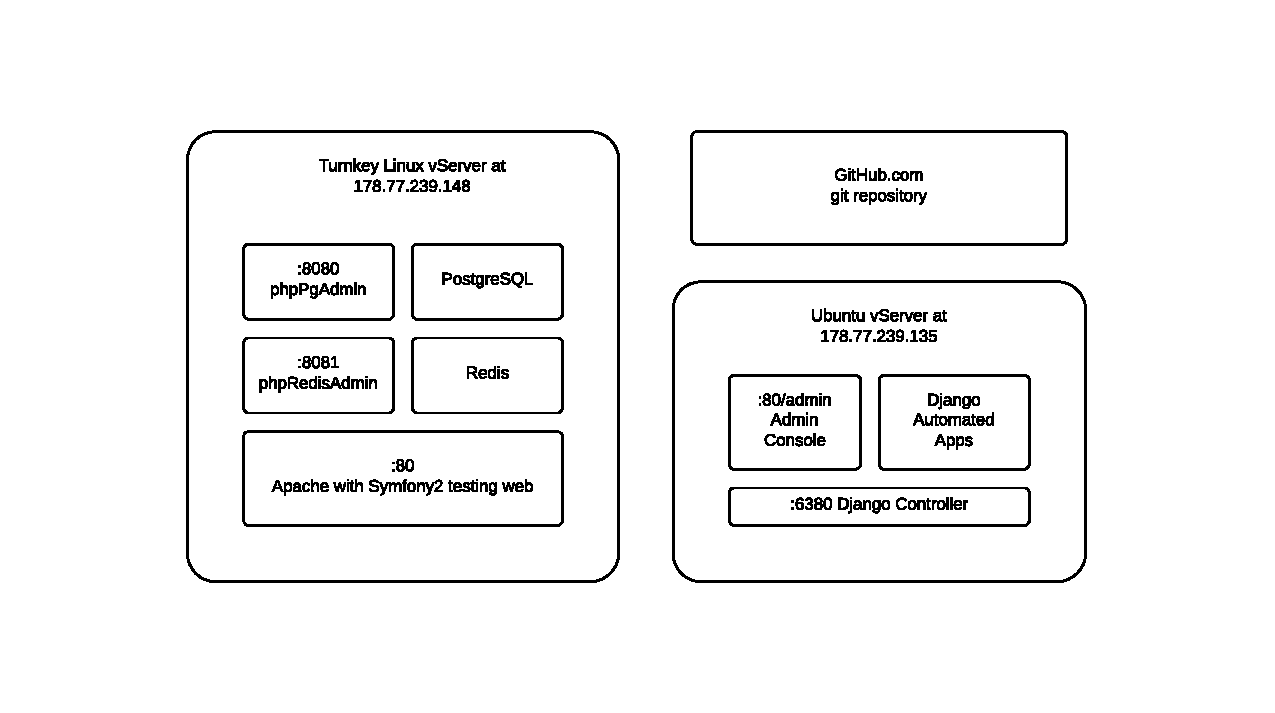
\includegraphics[trim=2.5cm 2cm 3cm 2cm, clip=true, totalheight=190pt]{images/tndw-test.pdf}
	\caption{Testing environment}
	\label{fig: tndw-test}
\end{figure}

Testing environment is available at \url{http://alpha.thenewdistrowatch.eu}. Tryout of deployment and in-browser connection to one of the distributions is available at \url{http://alpha.thenewdistrowatch.eu/tndw-front/web/app_dev.php/distro/centos}. \\

Sources of this project are stored in three separate GIT repositories available at GitHub.com.

\begin{itemize}
	\item Frontend -- browsing at \url{https://github.com/jakubzitny/tndw-front}, cloning from \url{https://github.com/jakubzitny/tndw-front.git},
	\item Controller -- browsing at \url{https://github.com/jakubzitny/tndw-controller}, cloning from \url{https://github.com/jakubzitny/tndw-controller.git},
	\item Cloud gate -- browsing at \url{https://github.com/jakubzitny/tndw-back}, cloning from \url{https://github.com/jakubzitny/tndw-back.git}.
\end{itemize}

%%
%% RELEASE
%%
\chapter{Release and production environment}
\label{chapter:producion}

Production environment is based on the idea of one virtual server for every component. Separate machines will be running frontend web server and backend. Two other virtual servers will be dedicated for databases, one as primary and second one as backup. In case of the first one fails, there will be a load balancer to change their IP adresses, so the backup one is used as primary. Both database servers will have phpPgAdmin interface. Separate virtual server will be used for the Redis MQ and phpRedisAdmin. Proposed production environment is pitured on \hyperref[fig:tndw-prod]{figure 4.1}. \\

\begin{figure}[h!]
	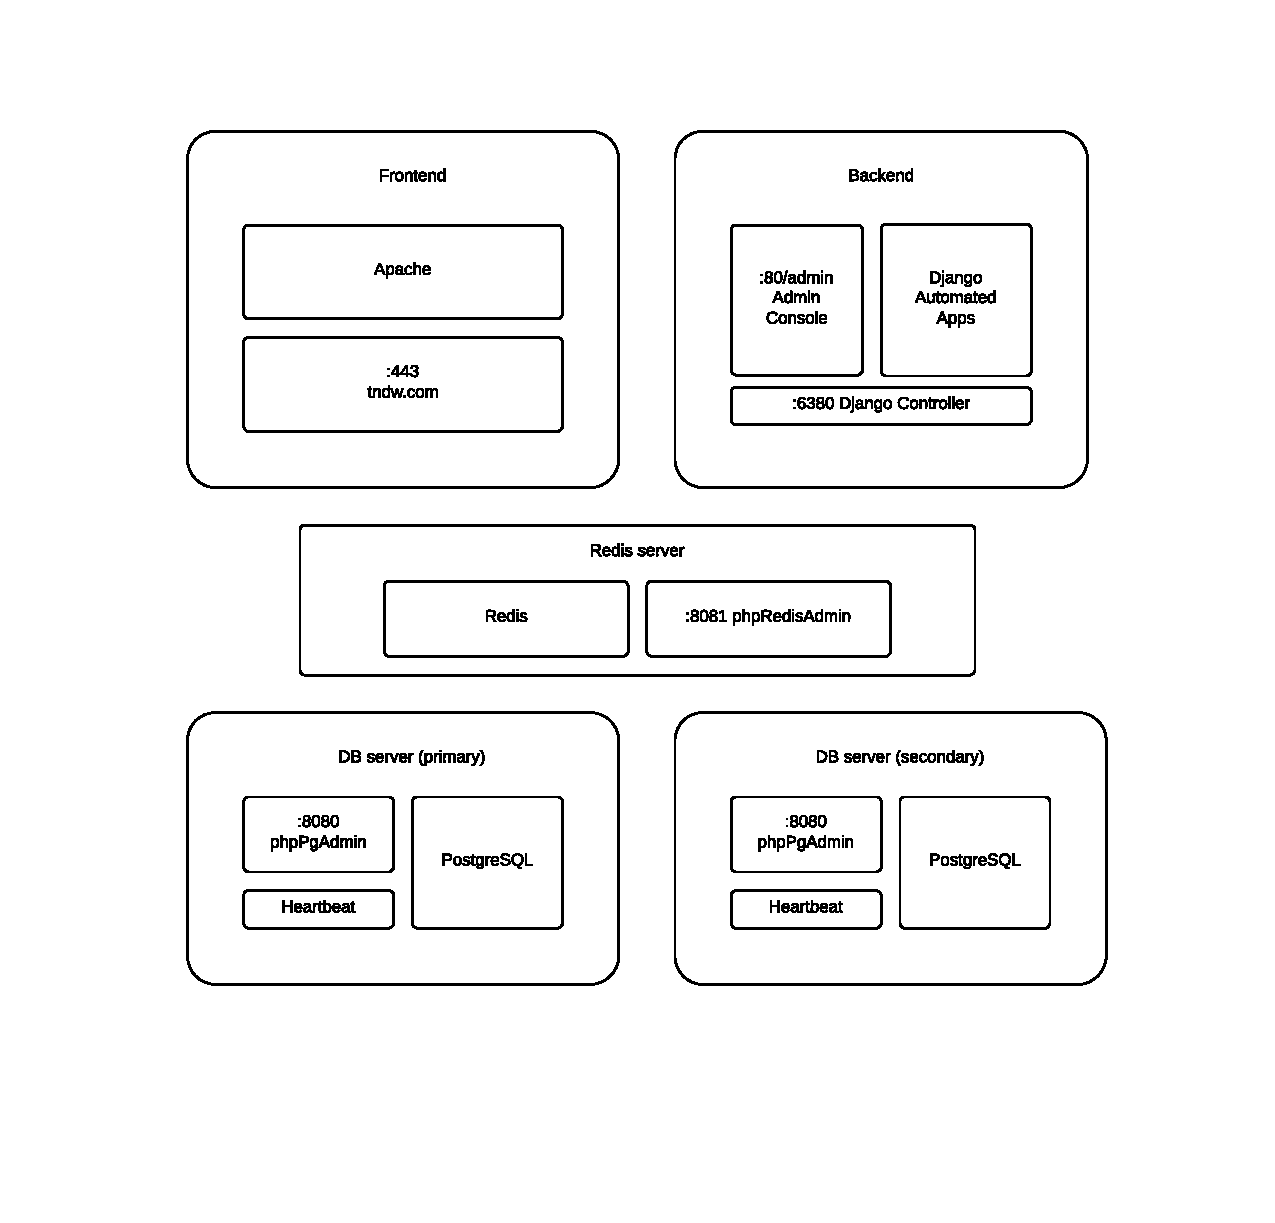
\includegraphics[trim=2.5cm 2cm 2.5cm 2cm, clip=true, totalheight=390pt]{images/tndw-prod.pdf}
	\caption{Production environment}
	\label{fig:tndw-prod}
\end{figure}

A lot of testing of previously described IaaS cloud projects has shown that the use of Openstack software would be the easiest and the most effective. However, to plug it in, one would need at least two physical machines with virtualization capabilities. If such resources were available, even load balancing techniques and further scaling the infrastructure would be possible. Production environment has not been set up as part of this thesis.

%%
%% CONCLUSION
%%
\begin{conclusion}
\label{chapter:conclusion}
This work has had a primary purpose to design and implement a system that will be fully automated and will offer a way to present and compare various operating systems. This part had been successfully completed. The system was designed with attention to detail and choosing the right tools for implementation. A lot of frameworks and libraries were also discussed and the result is ready to be expanded by further functionality.

Additionally, working on this required understanding of how open-source unix-like systems work in general, how it is possible to operate them automatically and what projects have already been digging into these matters. A lot of them are also outlined in this work. Few of the automated procedures from the backend component of this project could be also used in other works. They could be released as separate open-source projects. \\

On the other hand, there is still a lot of ideas to be implemented and finished more precisely. The project is designed to be easily expandable and it is not finished after submitting this thesis. In the future, I would like to add the following features:
\begin{itemize}
	\item Working with private IaaS cloud environments could be more precise. Resources need to be scaled in order to offer them for the general public. Also, linking with proprietary cloud providers can be really useful.
	\item This thesis and testing environment could be presented to people behind the original distrowatch.com. They may be interested in the frontend's graphical design or the backend automated procedures.
	\item It would also be great to provide pre-installed virtual disk images in different formats.
\end{itemize}

Although the system has been designed and implemented, it cannot be used to serve deployed operating systems in the cloud for many users. In order to really put this system for use in production environment, this project would need strong financial injection or server resources at least. Currently, only the testing environment is in the operation and launching operating systems is done via gate to IaaS cloud from T-Mobile available at \url{http://cloud.t-mobile.com}.

\end{conclusion}

\bibliographystyle{iso690}
\bibliography{mybibliographyfile}


\appendix

\printglossaries
\glsaddall

\chapter{Screenshots of the result}

\begin{center}
\begin{figure}[overhang]
	\advance\leftskip-0.75cm
	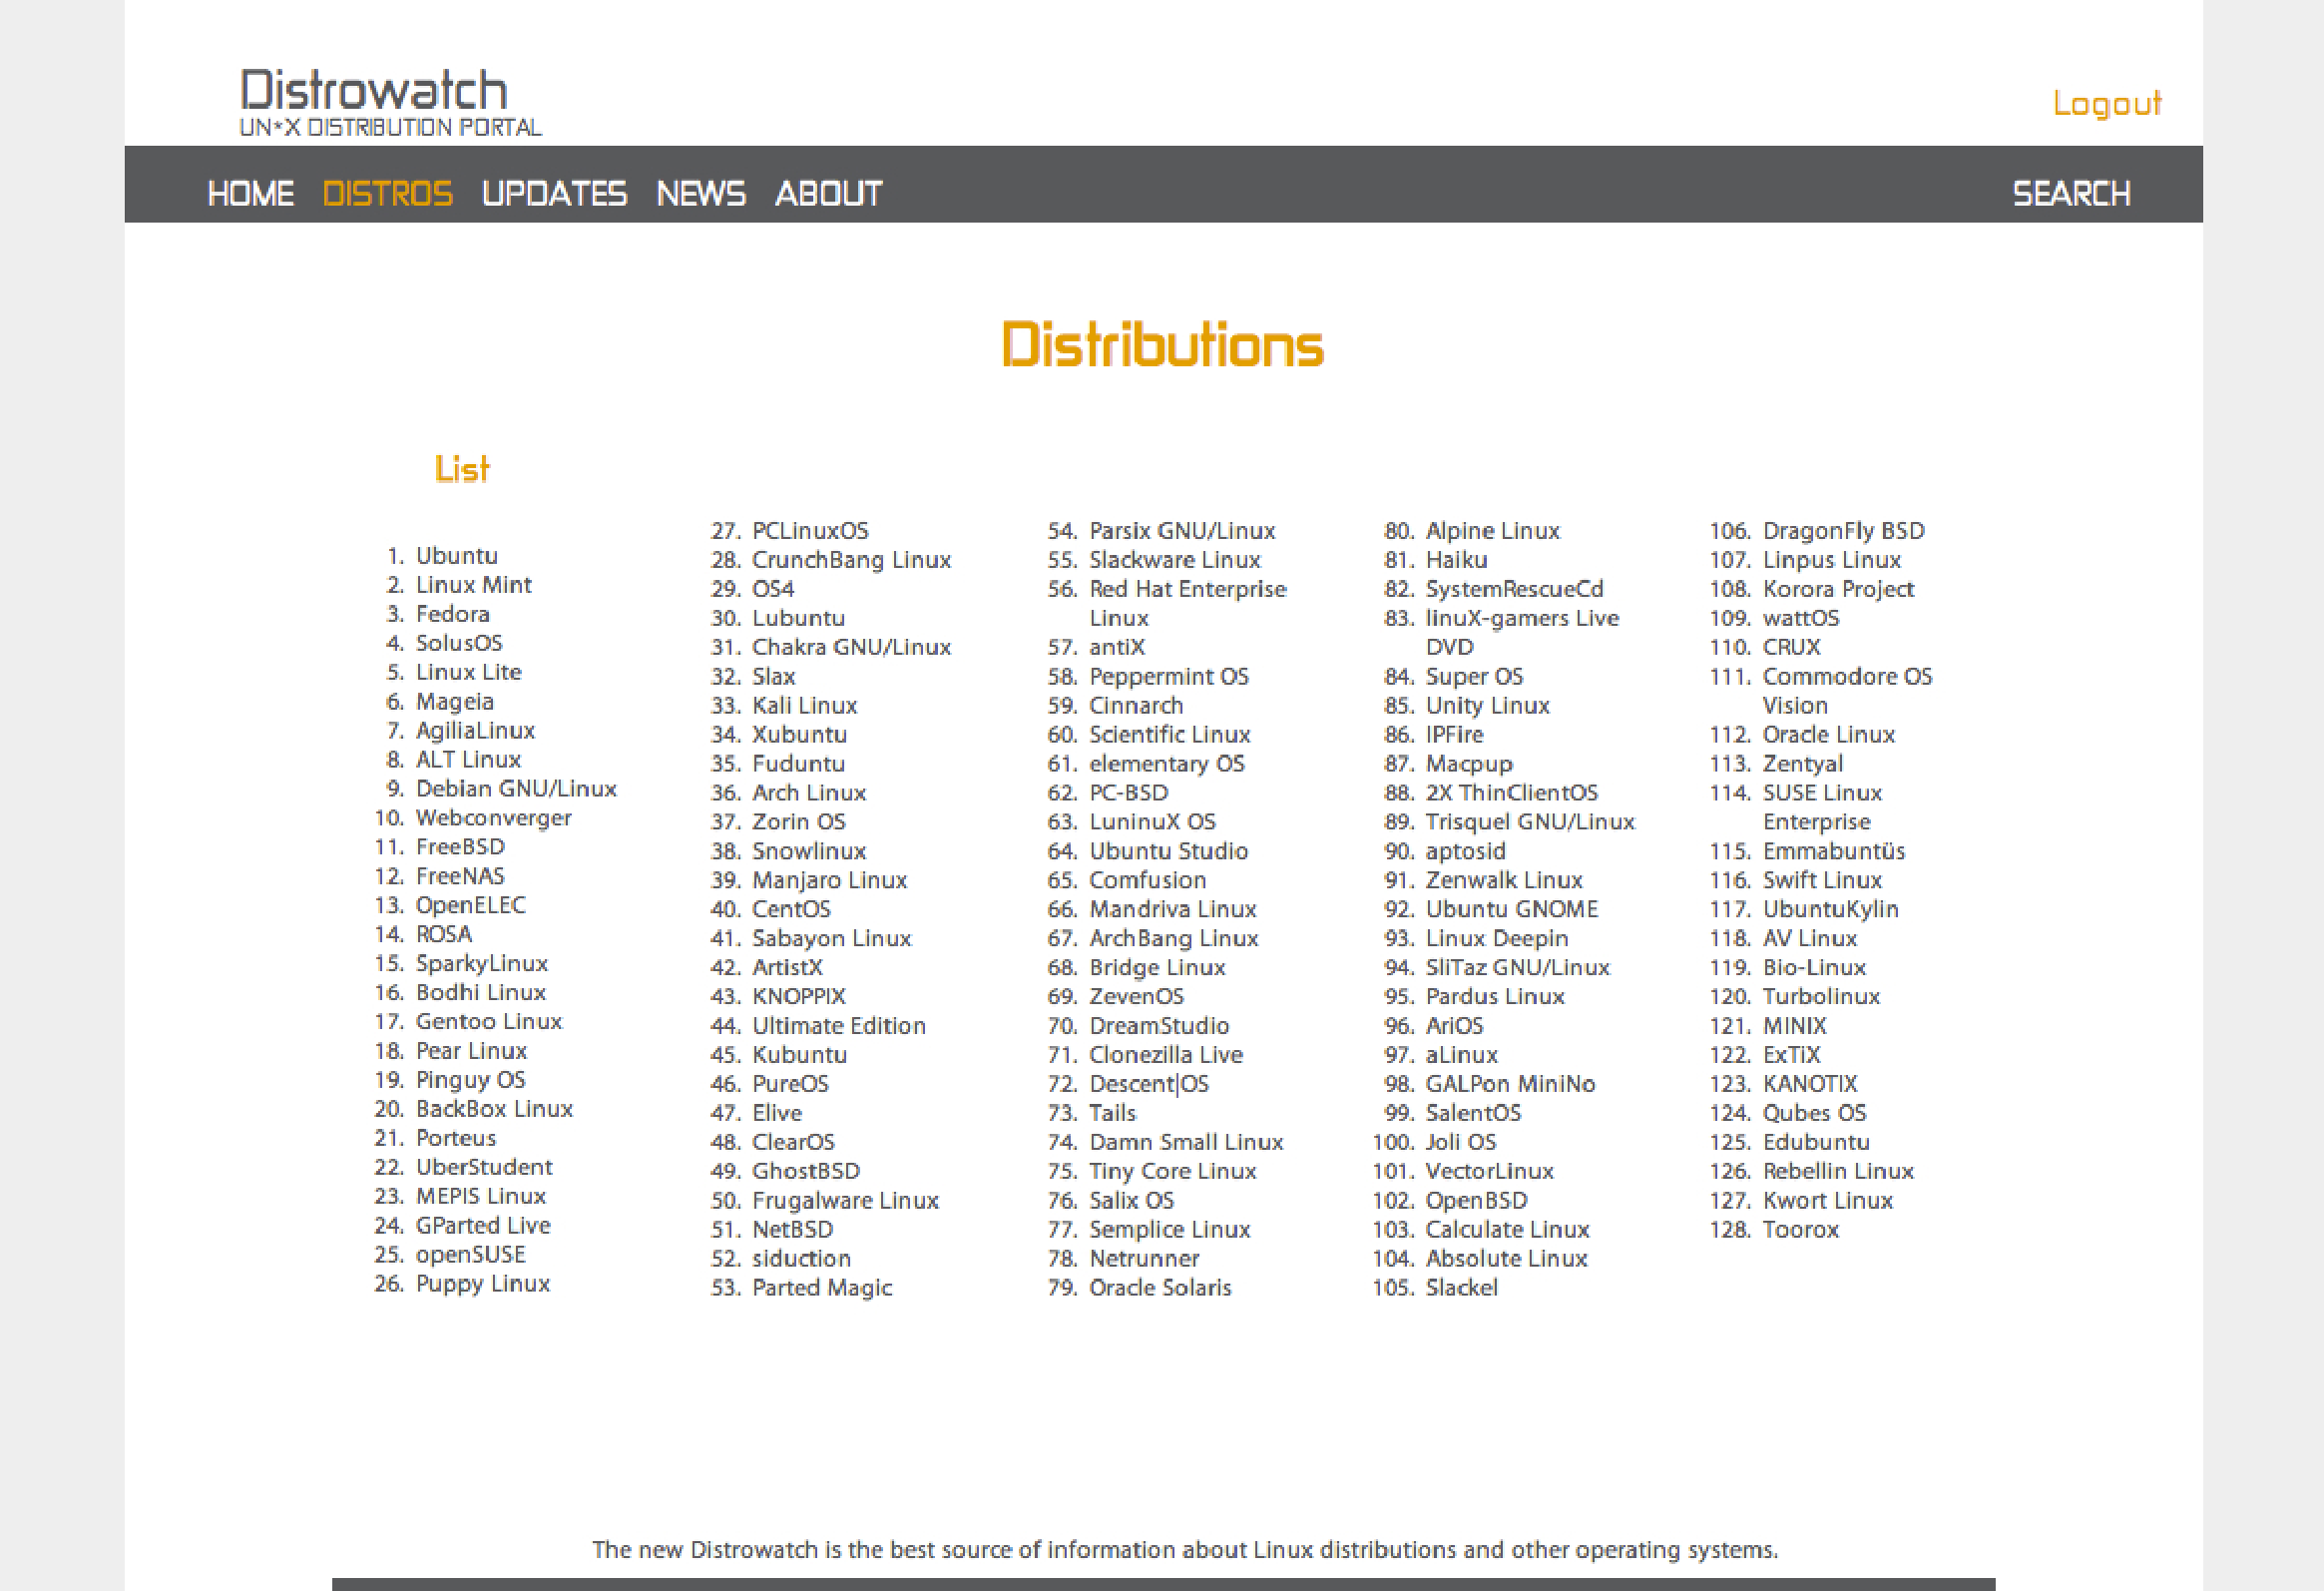
\includegraphics[width=430pt]{images/screen_distros.pdf}
	\caption{Screenshot of the page with list of all available distributions}
	\label{fig: tndw-screens}
\end{figure}

\begin{figure}[overhang]
	\advance\leftskip-0.75cm
	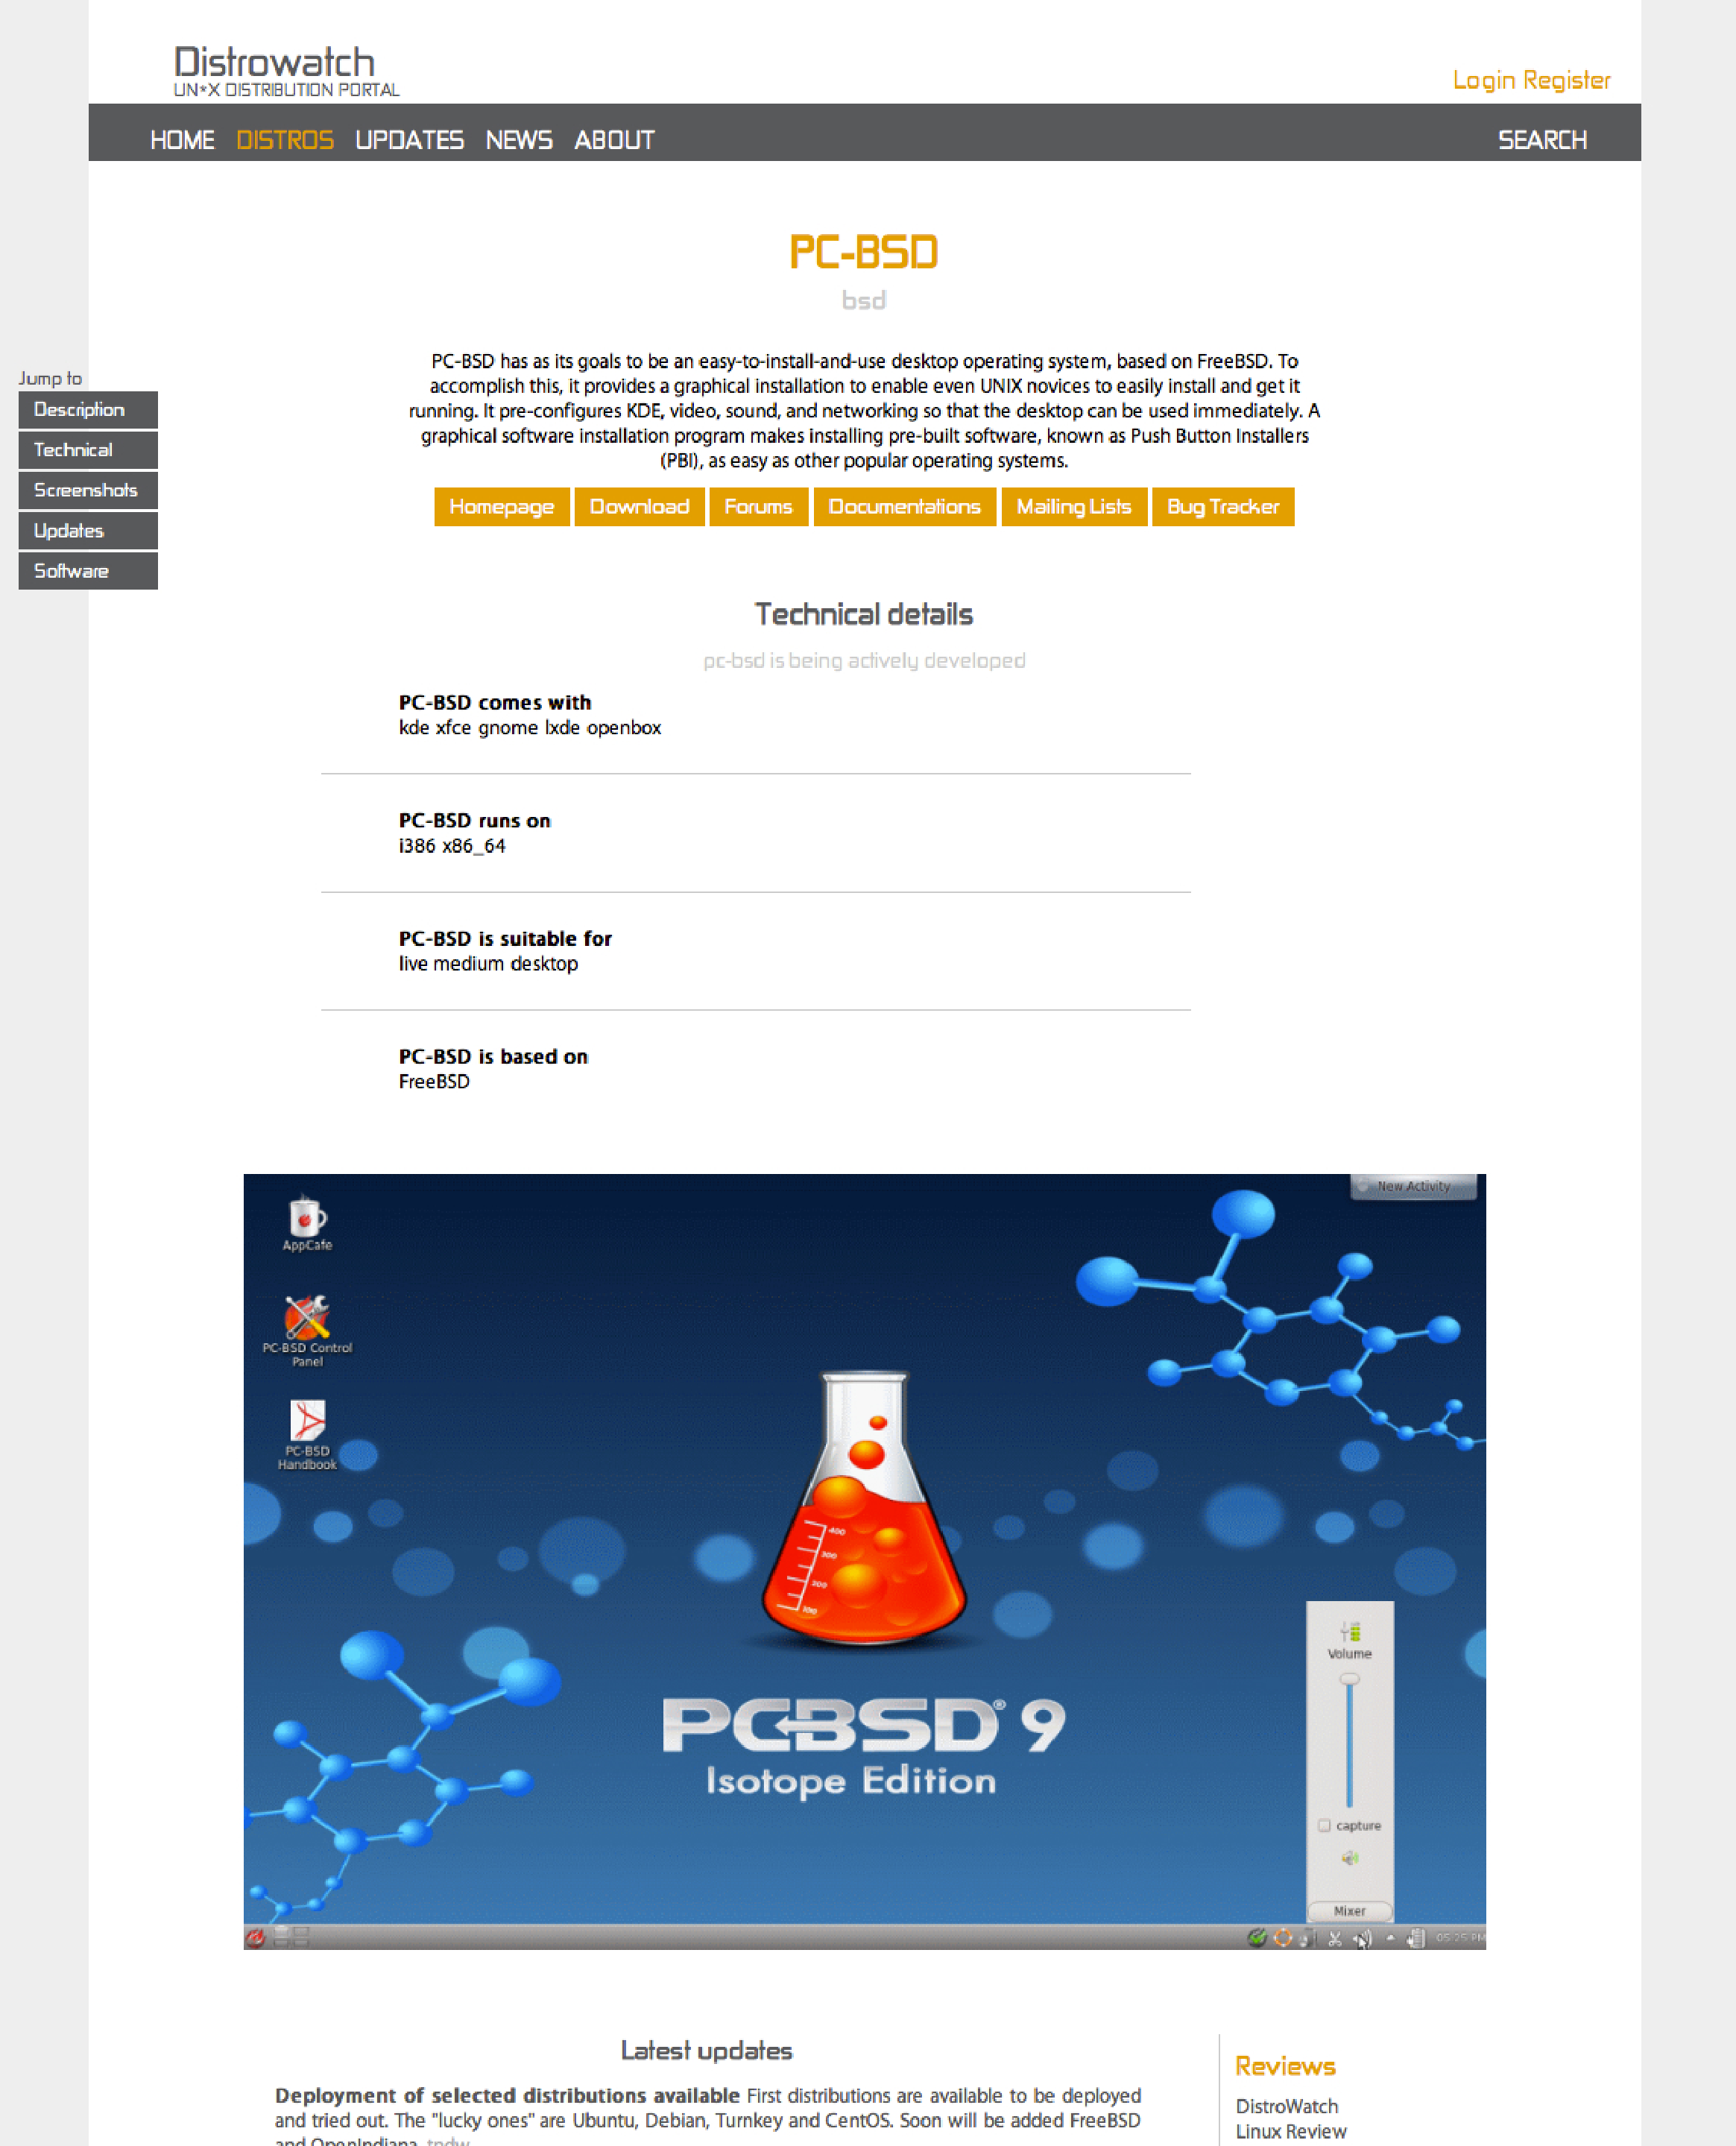
\includegraphics[width=430pt]{images/screen_pcbsd.pdf}
	\caption{Screenshot of the page about PC-BSD}
	\label{fig: tndw-screens}
\end{figure}

\begin{figure}[overhang]
	\advance\leftskip-0.75cm
	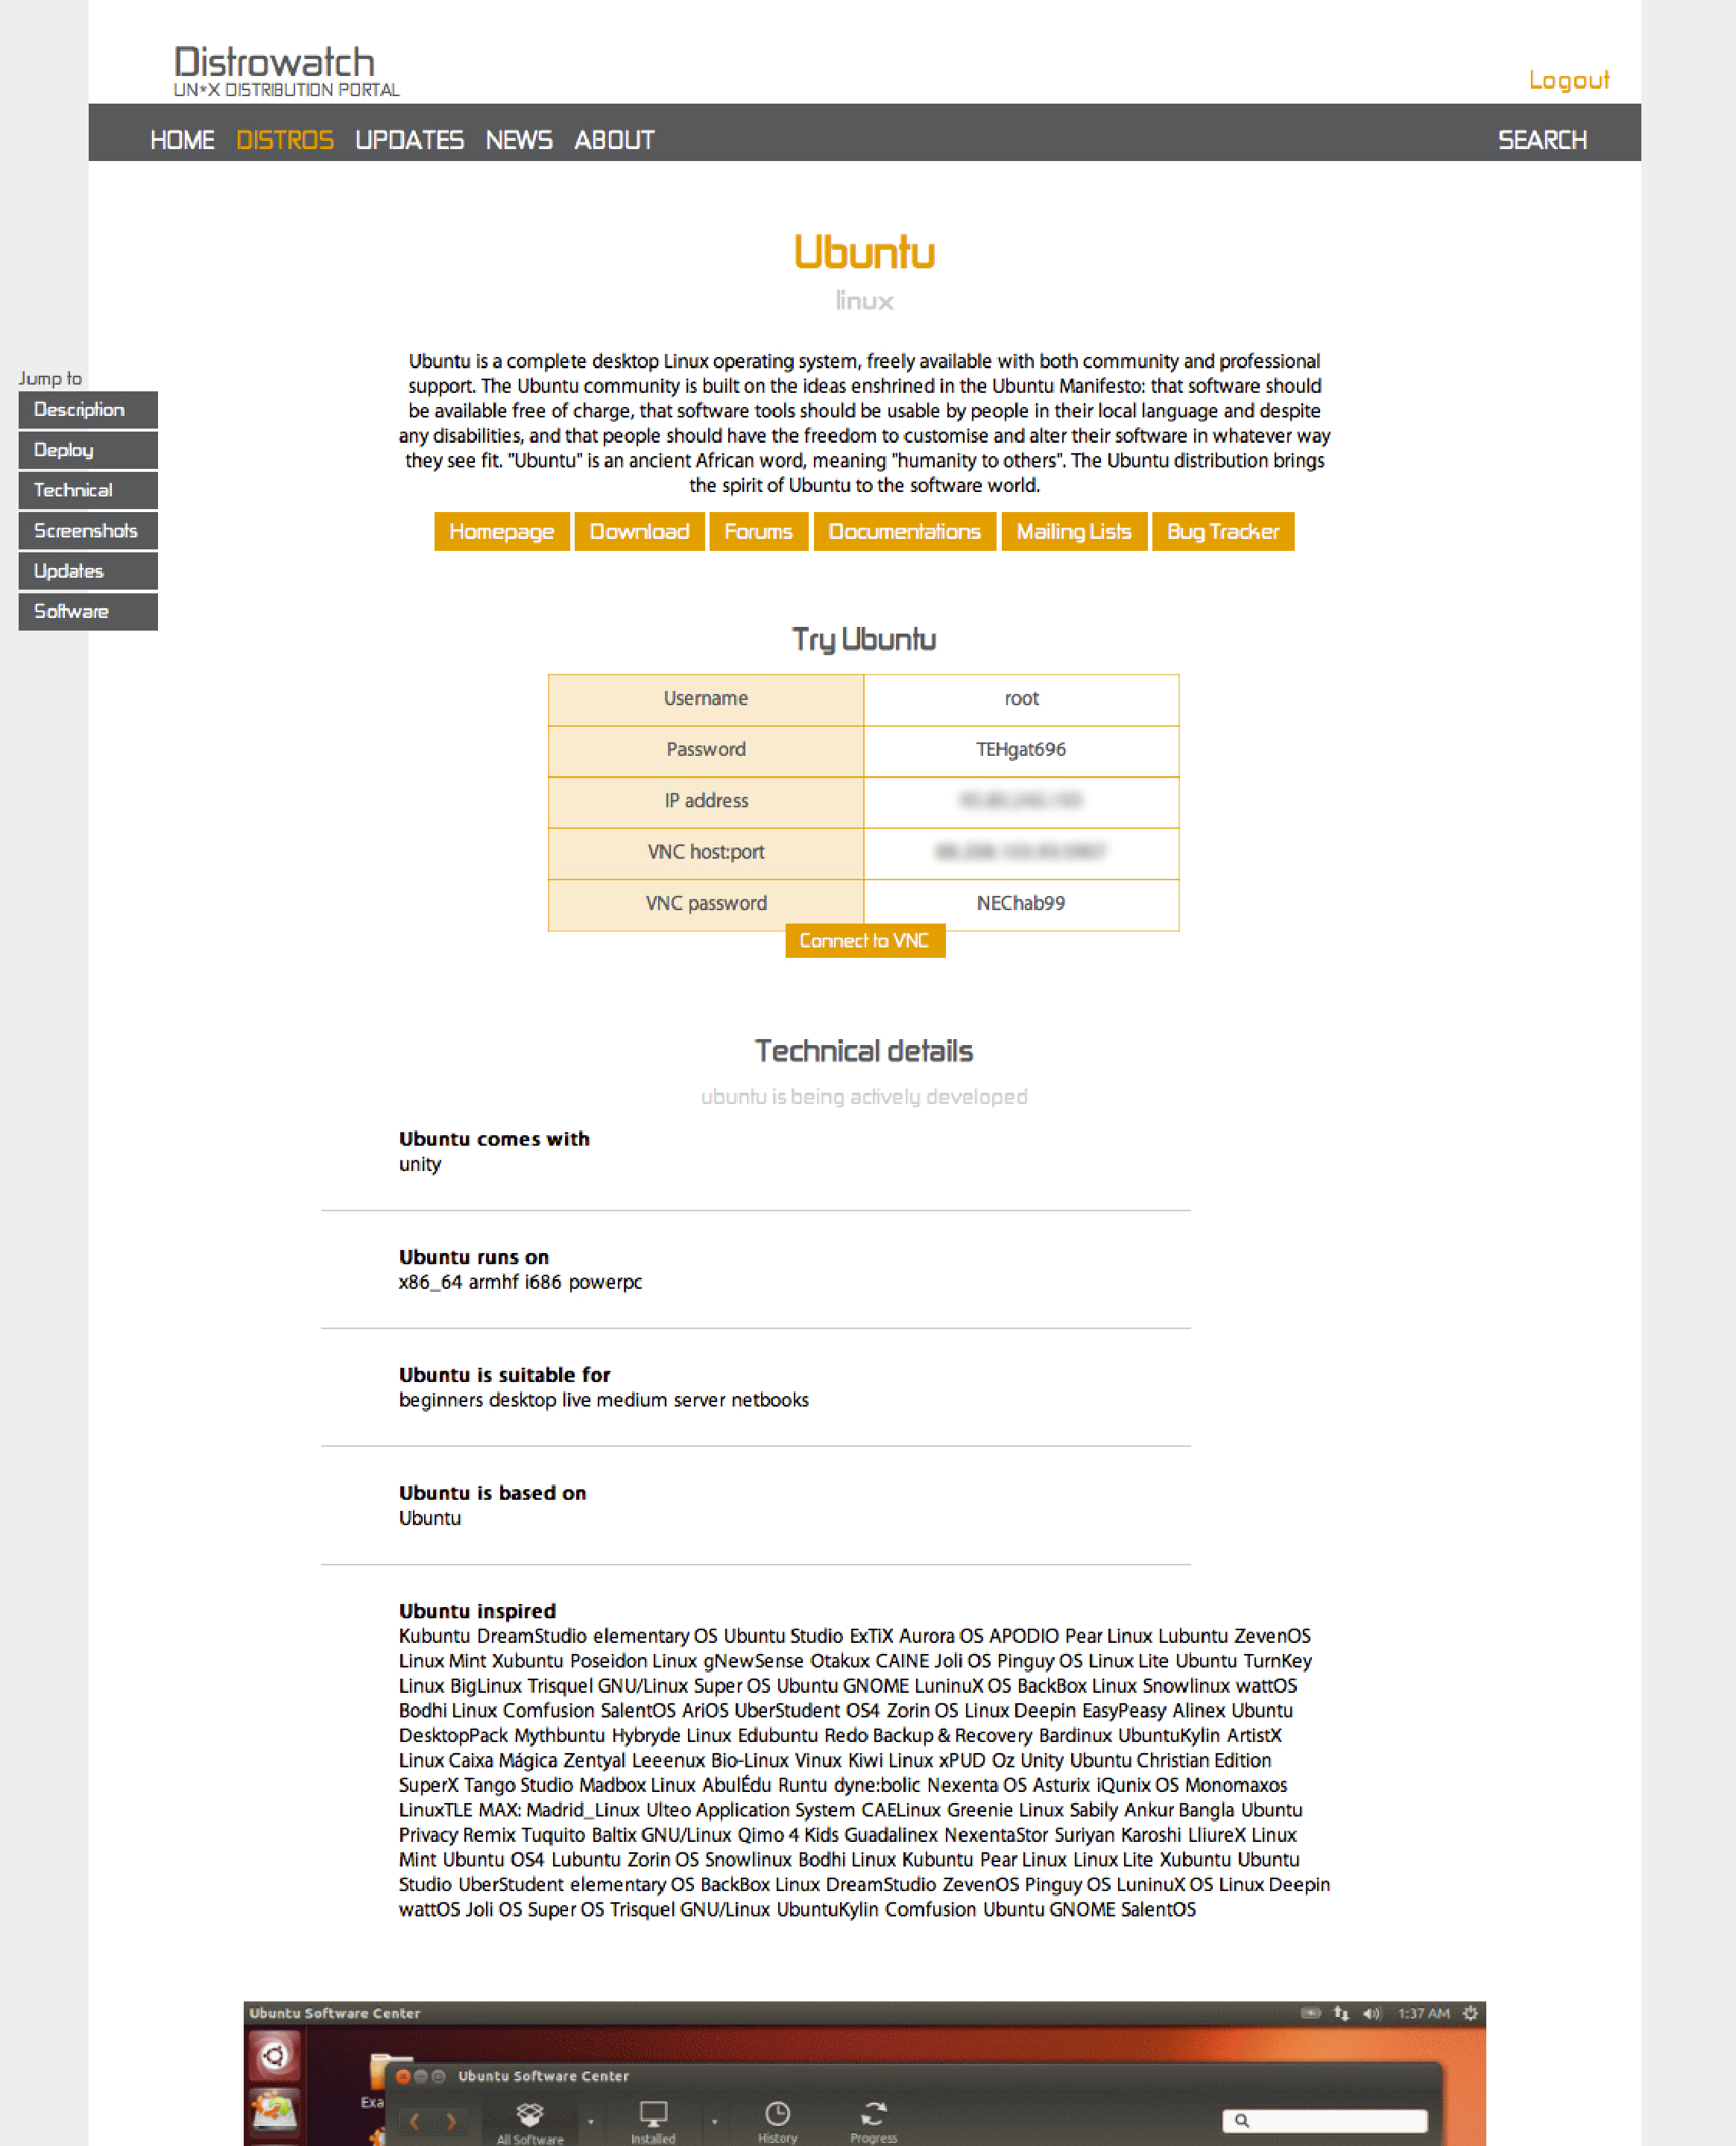
\includegraphics[width=430pt]{images/screen_ubuntu.pdf}
	\caption{Screenshot of the page about Ubuntu with deployed system}
	\label{fig: tndw-screens}
\end{figure}
\end{center}

\chapter{Software design}

\begin{figure}[h!]
	\advance\leftskip 0cm
	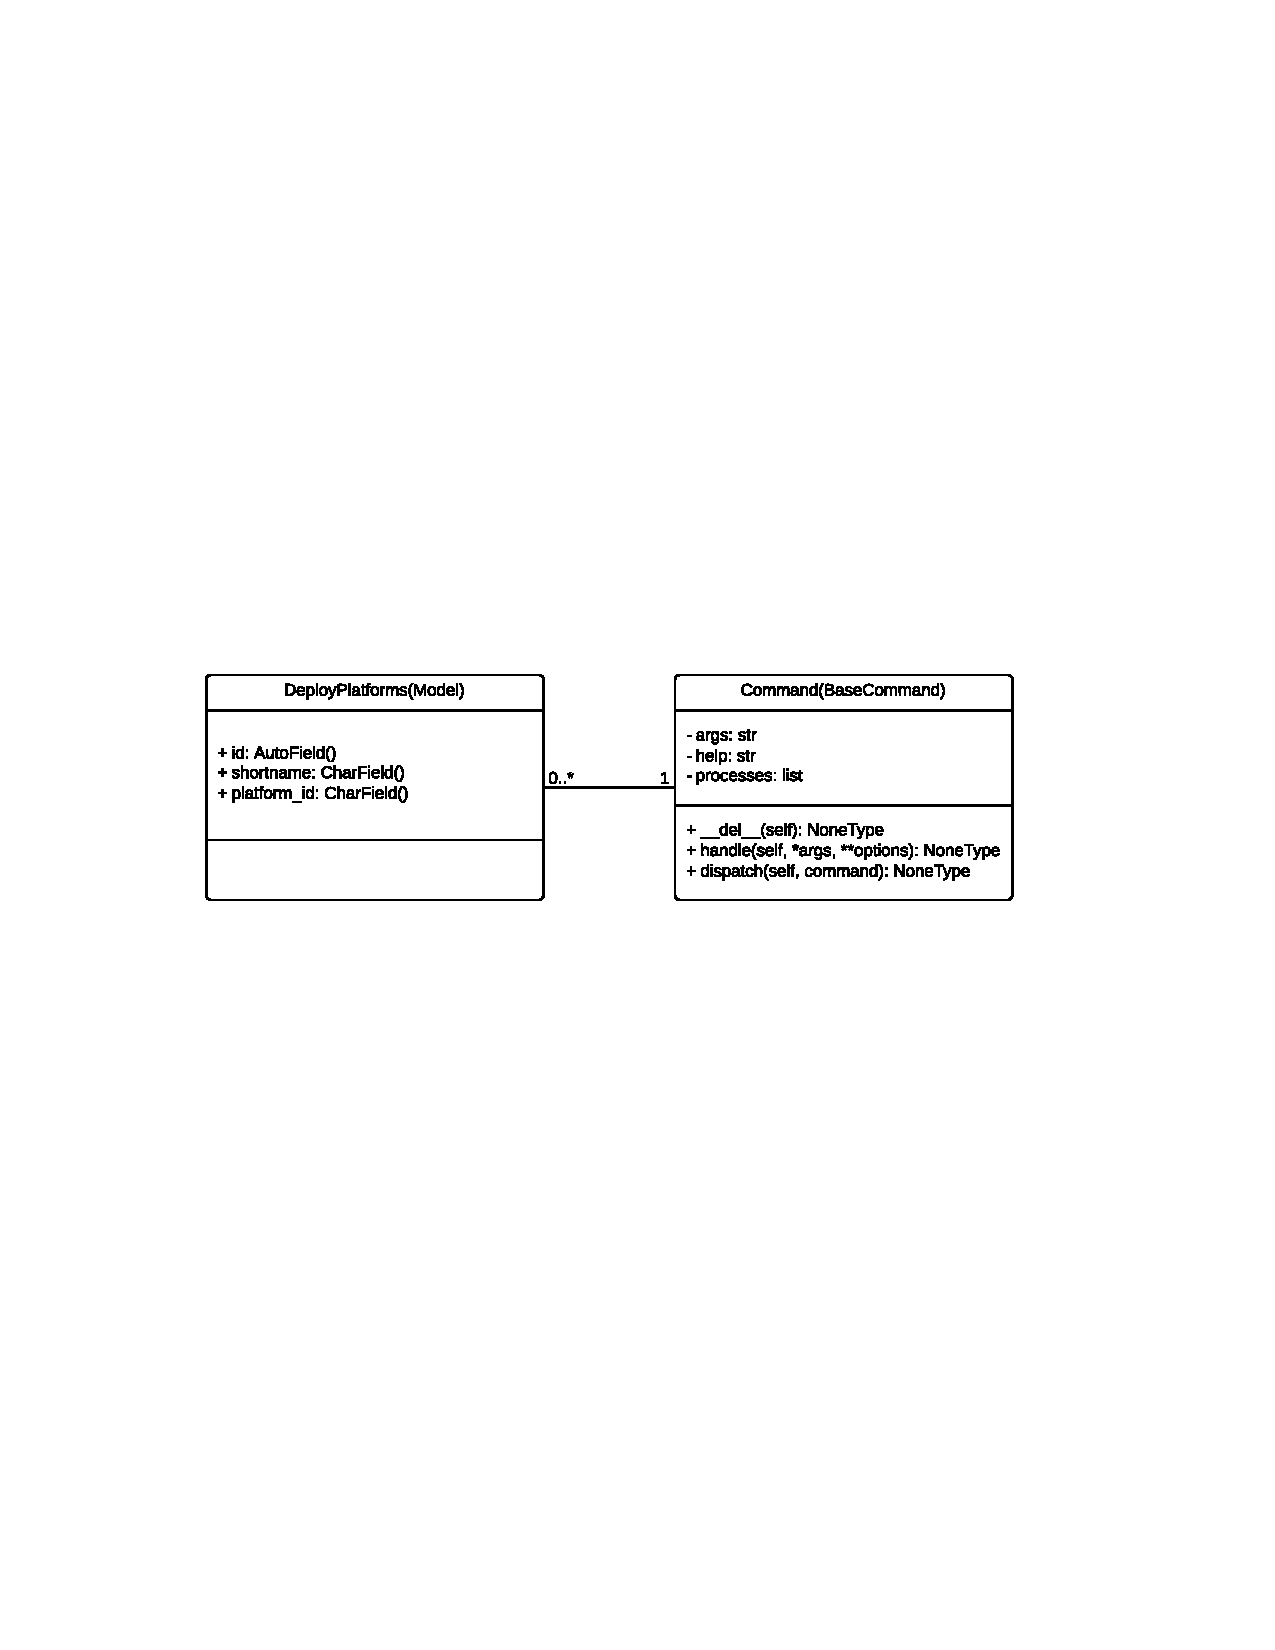
\includegraphics[trim=3cm 12cm 3cm 4cm, clip=true, totalheight=300pt]{images/back_listener.pdf}
	\caption{Domain model of listener app}
\end{figure}

\begin{figure}[h!]
	\advance\leftskip 1cm
	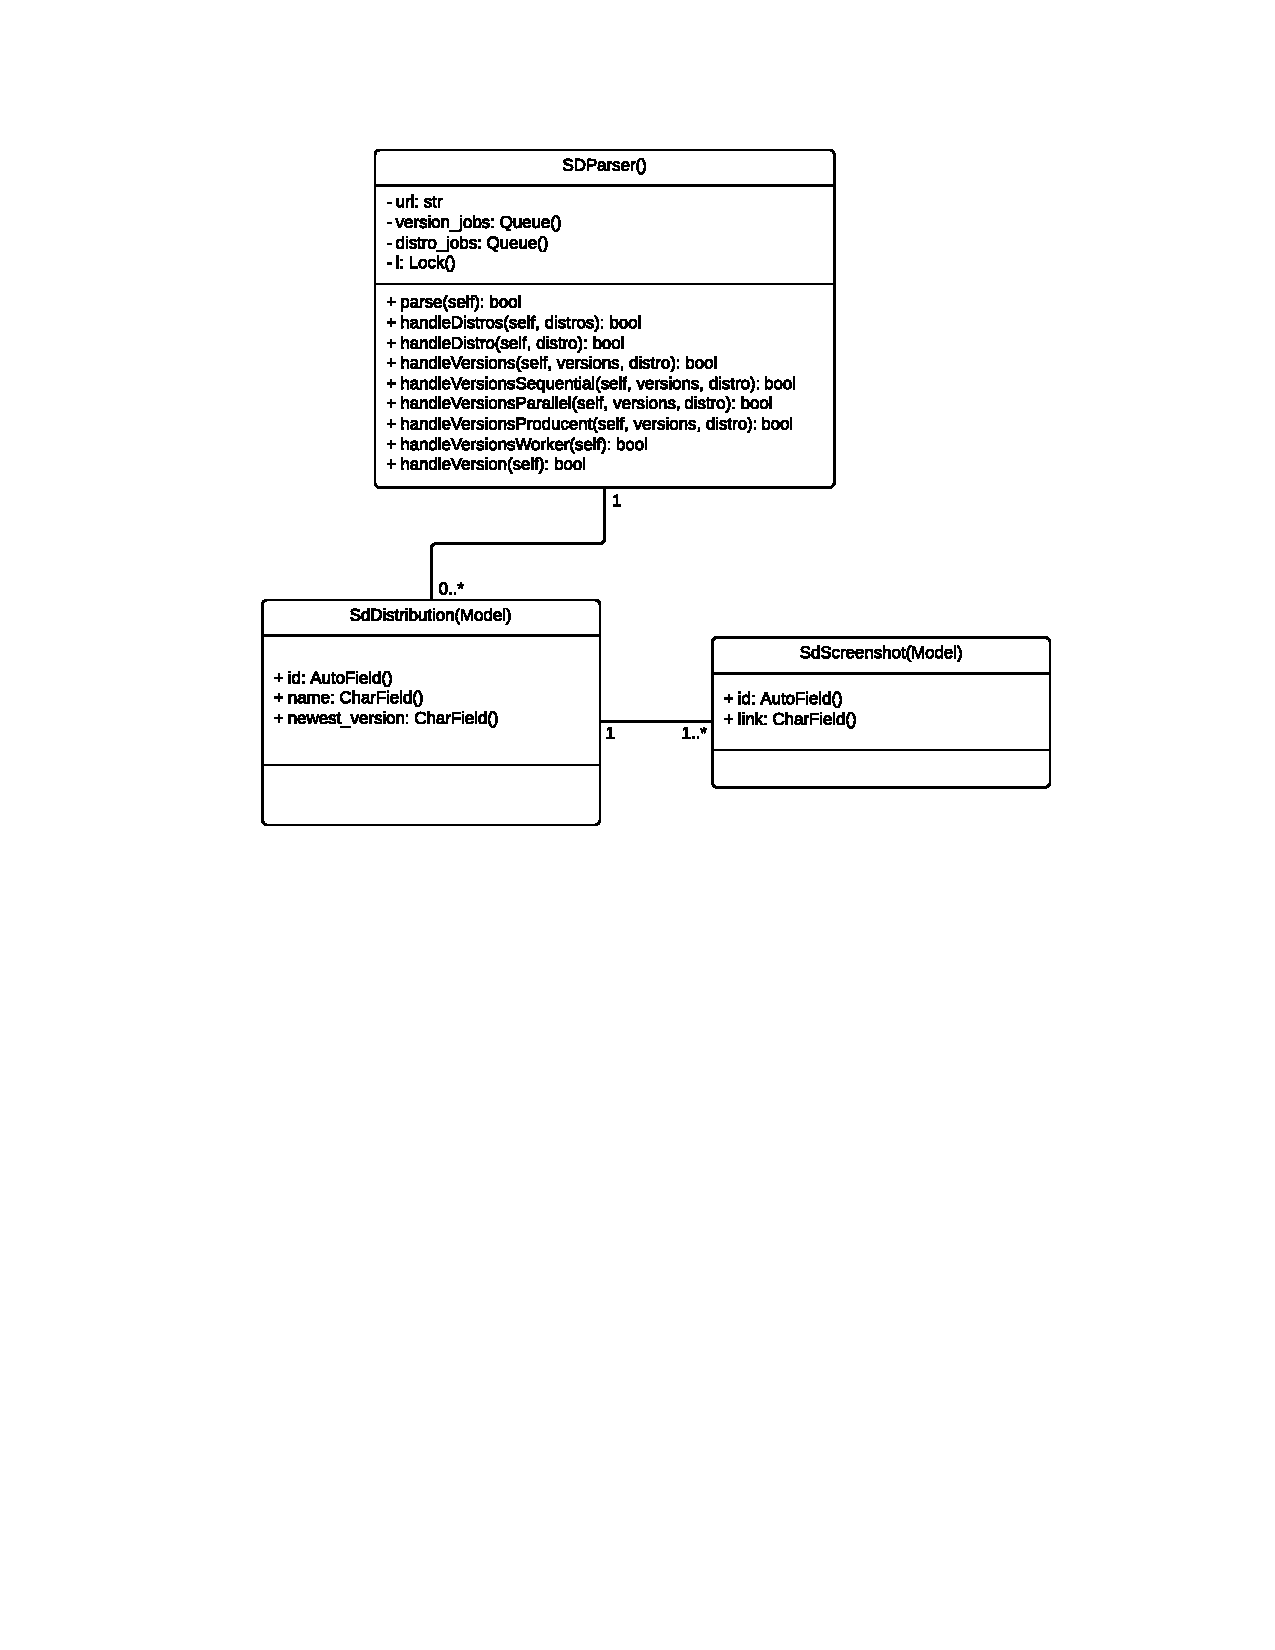
\includegraphics[trim=4cm 13cm 3cm 2cm, clip=true, totalheight=300pt]{images/back_screenshots_fetch.pdf}
	\caption{Domain model of screenshots\_fetch app}
\end{figure}

\begin{figure}[h!]
	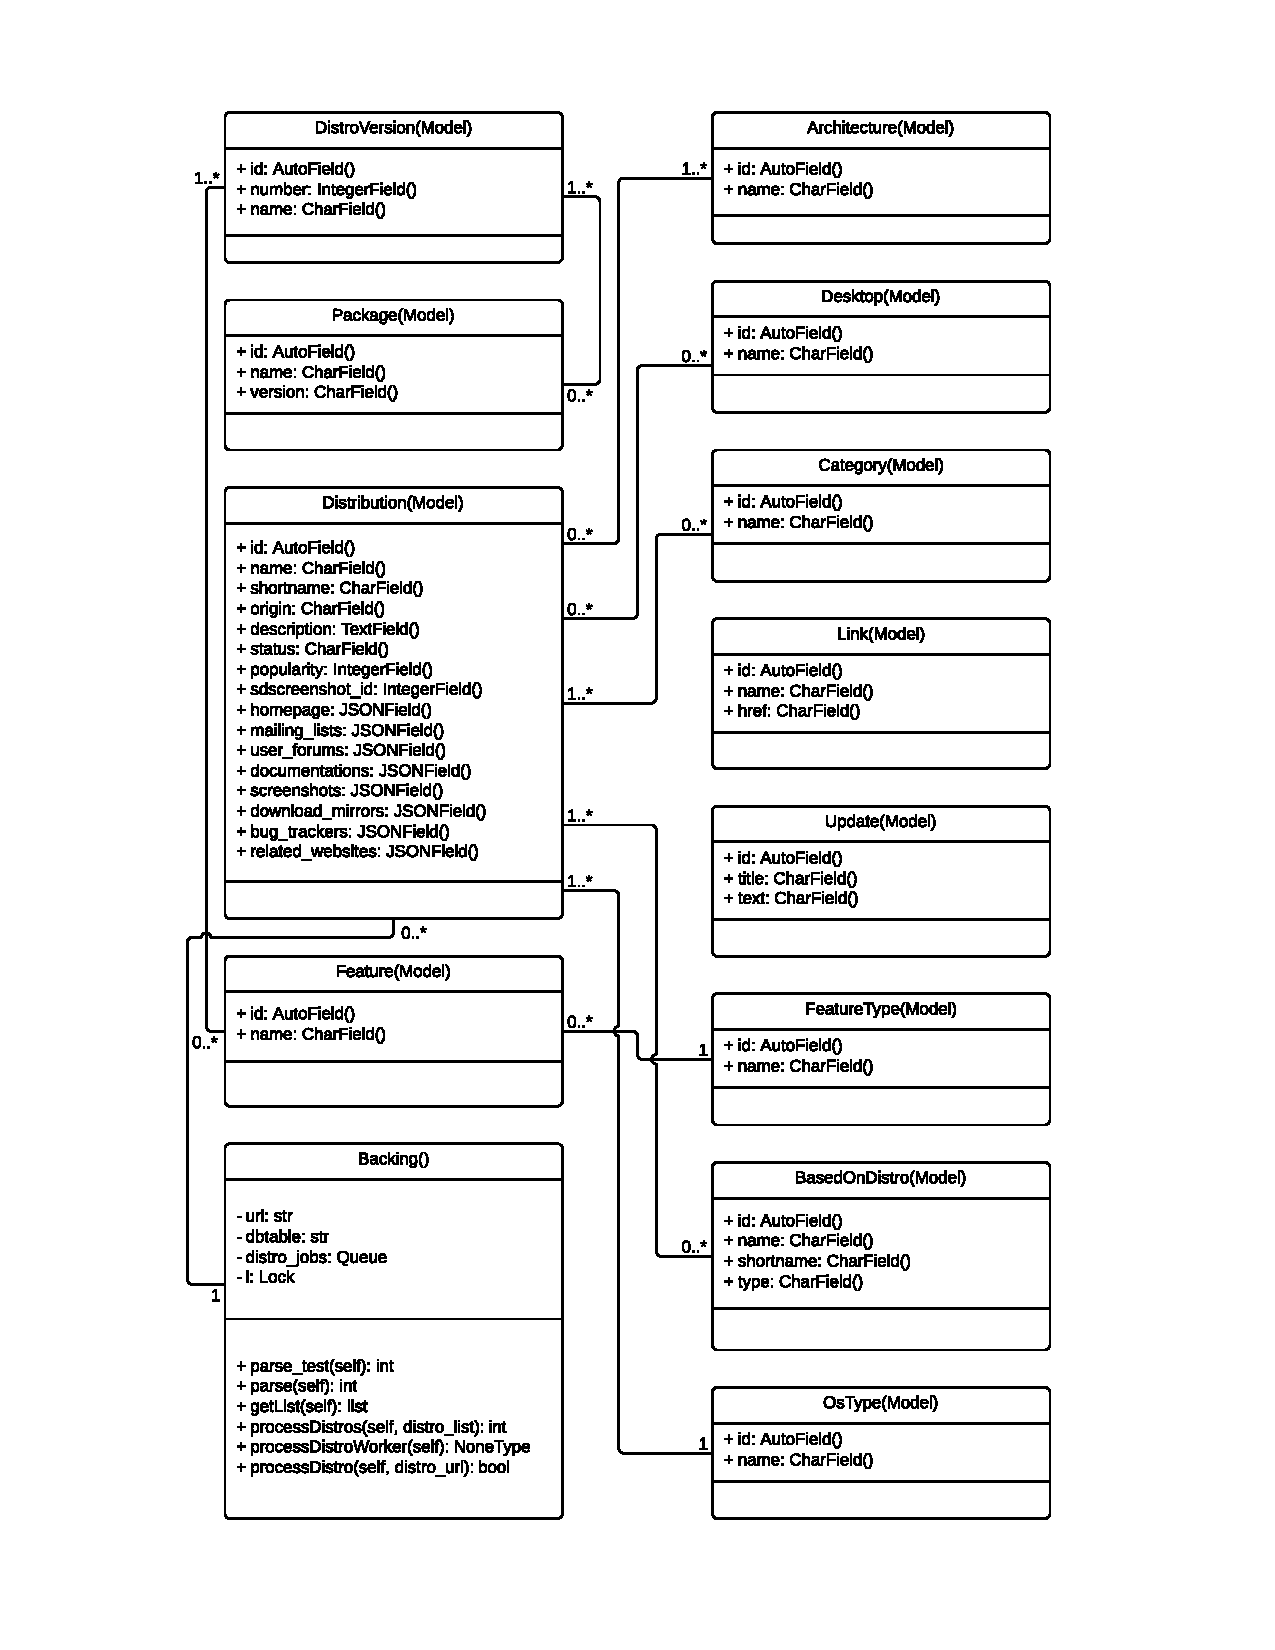
\includegraphics[trim=2.5cm 2cm 3cm 1cm, clip=true, totalheight=600pt]{images/back_backing.pdf}
	\caption{Domain model of backing app}
\end{figure}

\begin{figure}[h!]
	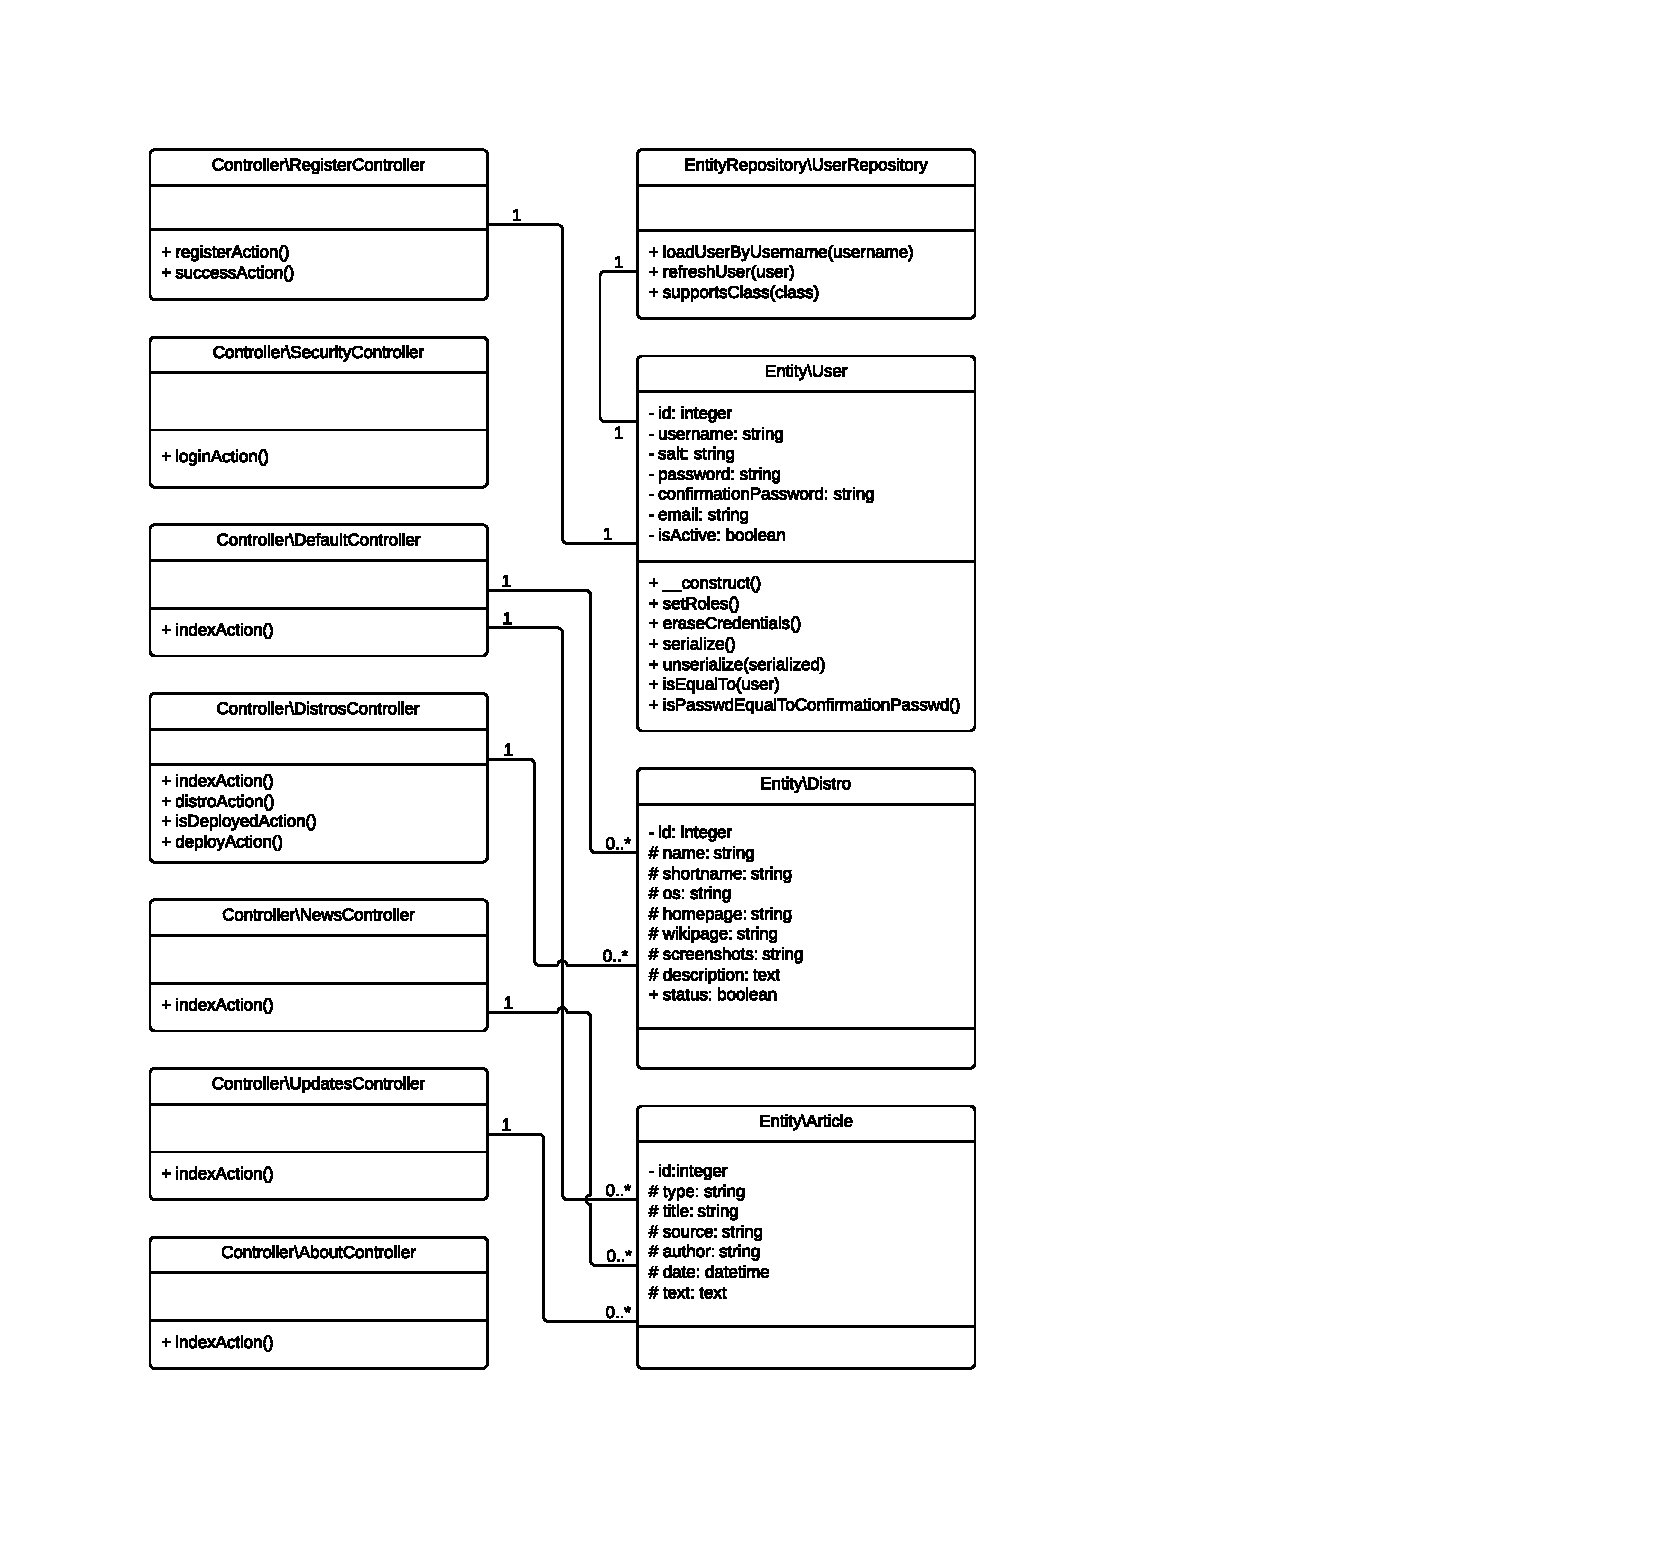
\includegraphics[trim=2.5cm 2cm 3cm 2.5cm, clip=true, totalheight=600pt]{images/tndw-front.pdf}
	\caption{Frontend's domain model}
\end{figure}

\chapter{CD contents}
\begin{figure}
	\dirtree{%
		.1 readme.txt\DTcomment{contents of the CD}.
		.1 sources.
		.2 tndw-front\DTcomment{frontend sources}.
		.2 tndw-controller\DTcomment{controller and backend sources}.
		.2 tndw-back\DTcomment{cloud gate sources}.
		.2 tndw-latex\DTcomment{thesis as \LaTeX \ sources}.
		.1 thesis\_zitny.pdf\DTcomment{thesis as PDF document}.
	}
\end{figure}

\end{document}
